

\chapter{Einleitung}\label{sec:Einleitung}

Das \emph{Semantic Web} erweitert das heutige Web um explizite Bedeutung: Inhalte werden so strukturiert, dass nicht nur Menschen, sondern auch Programme die Semantik verarbeiten und komplexe Aufgaben automatisiert unterstützen können \cite{bernersLee2001}. Dazu werden Informationen maschinenlesbar beschrieben (u.\,a.\ via URIs/IRIs und RDF-Tripeln), sodass Software-Agenten Datenquellen verbinden, Schlussfolgerungen ziehen und Dienste orchestrieren können—ohne zentrale Steuerung und im Sinne eines dezentralen, evolvierenden Webs \cite{bernersLee2001}.

Auf dieser Grundlage haben sich \emph{Wissensgraphen} als prägnante und flexible Datenabstraktion etabliert: Knoten repräsentieren Entitäten, Kanten ihre (auch komplexen) Relationen; Schemaentscheidungen können aufgeschoben, Datenquellen schrittweise integriert und Beziehungen über Pfade navigiert werden \cite{hogan2021}. Für RDF-basierte Wissensgraphen stellt \emph{SPARQL} die standardisierte Abfrage- und Änderungs\-sprache bereit. SPARQL operiert über Graphmuster (\emph{Basic Graph Patterns}) und unterstützt u.\,a.\ optionale/alternative Muster, Filter, Aggregation, Unterabfragen, Eigenschaftspfade sowie verschiedene Abfrageformen (SELECT, CONSTRUCT, ASK, DESCRIBE) \cite{w3cSparql11}. Trotz dieser Ausdrucksstärke bringt SPARQL inhärente Komplexität mit sich: Formal basiert es auf Graph-Matching; optionale Teile, UNION, FILTER, Projektion, DISTINCT/ORDER/LIMIT \emph{etc.} erhöhen die kognitive und algorithmische Schwierigkeit \cite{perezGutierrezSparql}. Für viele Endnutzer:innen bleibt die Syntax—und das Denken in Tripeln, Mustern und Bindungen—eine Hürde.

Parallel vergrößern \emph{Large Language Models (LLMs)} den Gestaltungsspielraum natürlicher Schnittstellen. GPT-4 zeigt, dass Modelle natürliche Sprache robust verarbeiten und in anspruchsvollen Benchmarks Leistungsniveaus nahe menschlicher Expert:innen erreichen können—bei bekannten Grenzen wie Halluzinationen und der Notwendigkeit geeigneter Sicherheitsmaßnahmen \cite{openaiGPT42023}. Dies legt nahe, natürliche Sprache als Interface zu RDF-Daten nutzbar zu machen: Benutzer:innen formulieren Aufgaben in Alltagssprache; ein LLM generiert daraus \emph{valide} SPARQL-Operationen.

Für reale, domänenspezifische Wissensgraphen (z.\,B.\ historische Personen, Orte, Organisationen) genügt es jedoch nicht, nur SELECT-Anfragen abzudecken. Gefordert ist die \emph{semantische Bearbeitung}—\textbf{INSERT}, \textbf{DELETE} und \textbf{UPDATE}—mit \emph{Nachvollziehbarkeit} und \emph{Sicherheit}. Dabei ist der \textbf{Datenschutz} zentral: Bei natürlicher Spracheingabe, Prompt-Kontext und beim Logging können personenbezogene Daten betroffen sein; die EU-DSGVO fordert u.\,a.\ Datenminimierung, Zweckbindung, Integrität/Vertraulichkeit und Rechenschaftspflicht \cite{euGDPR2016}. Privacy-by-Design ergibt sich hier u.\,a.\ durch die Beschränkung des Modellkontexts auf \emph{Ontologie statt Instanzdaten} sowie durch Pseudo\-nymisierung und strikte Aufbewahrungsregeln für Query-Logs.

\paragraph{Ziel der Arbeit.}
Diese Arbeit konzipiert, implementiert und evaluiert eine Schnittstelle, die \emph{natürliche Sprache} in \emph{valide SPARQL-Änderungsoperationen} überführt und Datenschutz sowie Nachvollziehbarkeit durchgängig verankert. Kernideen sind:
\begin{enumerate}
\item LLM-gestützte Generierung mit \emph{Ontologie-Kontext} (Klassen/Properties) statt vollständiger Instanzdaten,
\item \emph{Vorschau} und \emph{Erklärung} der betroffenen Tripel,
\item \emph{schrittweise Bestätigung} und \emph{Undo},
\item \emph{Protokollierung} mit Pseudonymisierung und klaren Lösch-/Aufbewahrungsregeln.
\end{enumerate}

\paragraph{Eigene Beiträge.}
Gegenüber bestehenden NL{\textrightarrow}SPARQL-Ansätzen fokussiert diese Arbeit drei miteinander verzahnte Neuerungen: (i) ein Ontologie-only-Prompting, das personenbezogene Instanzdaten konsequent aus dem LLM-Kontext heraushält, (ii) ein zweistufiger Preview/Execute-Workflow mit bestätigungspflichtigem Token, Explainability und deterministischen Undo-Queries, sowie (iii) ein Logging-Konzept, das Pseudonymisierung und Privacy-by-Design-Metadaten (DPV) kombiniert. Die Architektur und Referenzimplementierung wurden vollständig vom Autor entwickelt und in eine produktionsnahe Entwicklungsumgebung der Pfarrerdatenbank überführt. In der Evaluation (Kapitel~\ref{sec:evaluation}) werden diese Bausteine gemeinsam betrachtet und gegenüber Anforderungen aus Datenschutz, Governance und Usability reflektiert.

\paragraph{Forschungsfragen.}
\begin{description}
\item[RQ1:] Mit welcher Genauigkeit lassen sich natürliche \emph{Änderungsanweisungen} in \emph{syntaktisch valide} und \emph{semantisch korrekte} SPARQL-Operationen (INSERT/DELETE/UPDATE) überführen?
\item[RQ2:] Wie wirken \emph{Privacy-by-Design}-Maßnahmen (Ontologie-Kontext, Pseudonymisierung von Logs) auf Datenschutz, Nachvollziehbarkeit und Nutzbarkeit?
\item[RQ3:] Wie beurteilen Nutzer:innen die \emph{Benutzbarkeit} (Verständlichkeit von Vorschau/Erklärungen/Undo) im Vergleich zu handgeschriebenen Queries; welcher Overhead entsteht?
\end{description}

\paragraph{Beitrag und Aufbau.}
Die Arbeit liefert (i) eine \emph{Anforderungsanalyse} für NL{\textrightarrow}SPARQL-Änderungen unter DSGVO-Vorgaben, (ii) eine \emph{Architektur} mit Komponenten für Prompting/Parser, Generator, Validator, Executor, Logger und Visualizer, (iii) eine \emph{Referenzimplementierung} (Frontend/Backend, SPARQL-Endpoint) und (iv) eine \emph{Evaluation} auf einer domänennahen Wissensbasis. Kapitel~\ref{sec:theorie} fasst Grundlagen (RDF/OWL/SPARQL, LLMs, Datenschutz) zusammen; Kapitel~\ref{sec:related-work} diskutiert verwandte Arbeiten; Kapitel~\ref{sec:konzeption} beschreibt Anforderungsanalyse \& Konzeption; Kapitel~\ref{sec:implementierung} die Implementierung; Kapitel~\ref{sec:evaluation} die Evaluation; Kapitel~\ref{sec:fazit} schließt mit Fazit und Ausblick.






\chapter{Theoretischer Hintergrund}
\label{sec:theorie}

\section{Grundlagen des Semantic Web}
\label{sec:grundlagen-semantic-web}

\subsection{Motivation und Grundidee}

Das World Wide Web ist allgegenwärtig und wächst stetig; seine Stärken -- hohe Aktualität, globale Verfügbarkeit und niedrige Publikationsschwellen -- gehen zugleich mit Herausforderungen einher: heterogene Formate, fehlende Qualitätssicherung und vor allem eine \emph{mangelnde maschinelle Interpretierbarkeit} von Inhalten \cite{Hitzler}. Suchmaschinen mildern dies mit statistischen Verfahren, bleiben jedoch letztlich stichwort- statt bedeutungsbasiert. 

Die Idee des \emph{Semantic Web} (SW) ist, Informationen \emph{von vornherein} so zu repräsentieren, dass sie von Maschinen verarbeitet, zusammengeführt und logisch erschlossen werden können -- interoperabel durch offene Standards wie RDF, RDFS, OWL und SPARQL \cite{Hitzler,AntoniouVanHarmelen}. Leitgedanke: \emph{Informationen so repräsentieren, dass Maschinen damit in menschlich nützlicher Weise umgehen können} \cite{Hitzler}.


\subsection{Globale Bezeichner: URIs/IRIs und Blank Nodes}

Interoperabilität setzt globale Identifizierbarkeit voraus. Dafür dienen URIs bzw. deren Internationalisierung IRIs, die Ressourcen und Eigenschaften eindeutig benennen; IRIs können in RDF an Subjekt-, Prädikat- und Objektposition auftreten; als Objekt sind alternativ Literale zulässig. Literale modellieren Basiswerte (mit Datentyp und optionalem Sprach-Tag). \emph{Blank Nodes} modellieren namenlose Hilfsknoten (nur Subjekt/Objekt) und sind nützlich für strukturierende Konstrukte, erschweren jedoch Identitätsabgleich und Abfragen über Datenquellen hinweg \cite{RDF11Primer,Hitzler}.

\subsection{RDF -- Datenmodell und Serialisierungen}
\label{subsec:rdf}

Das \emph{Resource Description Framework} (RDF) beschreibt Wissen als gerichtete Tripel
\(\langle\)\emph{Subjekt, Prädikat, Objekt}\(\rangle\) und formt daraus Graphen. RDF ist domänenneutral, dezentral komponierbar und fördert Wiederverwendung: Tripel aus verschiedenen Quellen lassen sich zusammenführen, sofern IRIs konsistent verwendet werden \cite{RDF11Primer,AntoniouVanHarmelen,Hitzler}.

\paragraph{Knotenarten.} (i) IRIs für Ressourcen und Eigenschaften; (ii) \emph{Literale} als Basiswerte mit Datentyp (typisch XSD) und optionalem Sprach-Tag; (iii) \emph{Blank Nodes} als namenlose Platzhalter \cite{RDF11Primer}.

\paragraph{Datensätze und benannte Graphen.} RDF erlaubt die Gruppierung mehrerer Graphen in Datensätzen (\emph{named graphs}) für Provenienz und Teilmengenbildung \cite{RDF11Primer}.

\paragraph{Serialisierungen.} Für Austausch und Lesbarkeit existieren mehrere Schreibweisen mit gleicher Semantik: \emph{Turtle} (menschlich gut lesbar), \emph{N-Triples/N-Quads} (zeilenbasiert, großskaliger Austausch), \emph{TriG} (Datensätze), \emph{JSON-LD} (JSON-native Einbettung) sowie \emph{RDFa} (Einbettung in HTML) \cite{RDF11Primer}.

\paragraph{Beispiel (Turtle).}
\begin{lstlisting}
@prefix ex:  <http://example.org/> .
@prefix xsd: <http://www.w3.org/2001/XMLSchema#> .

ex:SemanticWeb a ex:Buch ;
  ex:titel "Semantic Web – Grundlagen"@de ;
  ex:autor ex:Hitzler, ex:Kroetzsch, ex:Rudolph, ex:Sure ;
  ex:preis "42.00"^^xsd:decimal .
\end{lstlisting}

\paragraph{Vokabulare.} RDF selbst legt die \emph{Bedeutung} verwendeter Bezeichner nicht fest. Erst wohldefinierte Vokabulare und Ontologiesprachen präzisieren Semantik -- siehe RDFS/OWL \cite{Hitzler,AntoniouVanHarmelen}.

\subsection{RDFS -- Schematisierung und leichtgewichtige Inferenz}

\emph{RDF Schema} (RDFS) erweitert RDF um Basiskonzepte für Klassen und Eigenschaften, u.\,a.\ \texttt{rdfs:Class}, \texttt{rdf:Property}, Subklassen/Subproperties (\texttt{rdfs:subClassOf}/\texttt{rdfs:subPropertyOf}), sowie \texttt{rdfs:domain}/\texttt{rdfs:range} zur Typisierung von Subjekt/Objekt. Damit lassen sich eigene Vokabulare definieren und einfache Ableitungen (z.\,B.\ Typvererbung) durchführen \cite{RDFS11,Hitzler}.

\paragraph{Beispiel (Turtle).}
\begin{lstlisting}
ex:Universitaet rdfs:subClassOf ex:Institution .

ex:istVerheiratetMit a rdf:Property ;
  rdfs:domain ex:Person ;
  rdfs:range  ex:Person .

ex:istGluecklichVerheiratetMit
  rdfs:subPropertyOf ex:istVerheiratetMit .
\end{lstlisting}

RDFS ist ein \emph{universelles} Vokabular: Es beschreibt die Semantik der \emph{eigenen Begriffe} eines Domänenvokabulars, nicht die Domäne selbst. Ausdrucksstärke und Inferenz bleiben bewusst einfach und effizient \cite{RDFS11}.

\subsection{OWL~2 -- Ontologien und Schlussfolgern}
\label{subsec:owl}

Komplexere Abhängigkeiten überschreiten die Ausdruckskraft von RDFS. Die \emph{Web Ontology Language} (OWL~2) basiert auf Beschreibungslogiken und bietet reichhaltige Konstruktoren (Schnittmenge, Vereinigung, Komplement), Disjunktheit/Äquivalenz von Klassen, Kardinalitäten sowie Eigenschaften-Charakteristika (symmetrisch, transitiv, funktional etc.). Für verschiedene Praxisanforderungen existieren Profile (EL, QL, RL) mit garantierten Traktabilitätseigenschaften. \emph{OWL~DL} bleibt entscheidbar durch Typtrennung; \emph{OWL~Full} ist maximal ausdrucksstark, jedoch unentscheidbar \cite{Hitzler,AntoniouVanHarmelen,OWL2Overview}.

\paragraph{Skizze (RDF/XML-Ausschnitt).}
\begin{lstlisting}
<owl:Class rdf:about="ex:Professor"/>
<ex:Person rdf:about="ex:RudiStuder"/>
<owl:ObjectProperty rdf:about="ex:arbeitetGernMit"/>
\end{lstlisting}

\subsection{SPARQL~1.1 -- Abfragen über Graphen}
\label{subsec:sparql}

SPARQL fragt RDF als \emph{Graphmuster} ab; Tripelmuster enthalten Variablen (z.\,B.\ \texttt{?x}). Komplexe Muster entstehen durch Gruppierung, \texttt{OPTIONAL} (Left-Outer-Join), \texttt{UNION} (Alternativen) und \texttt{FILTER} (Bedingungen). \emph{Property Paths} erlauben Pfadnavigation beliebiger Länge. Ergebnisformen sind \texttt{SELECT}, \texttt{CONSTRUCT} (erzeugt RDF-Graphen), \texttt{ASK}, \texttt{DESCRIBE}. Modifikatoren wie \texttt{ORDER BY}, \texttt{LIMIT}/\texttt{OFFSET} und \texttt{DISTINCT} steuern Ausgabe \cite{SPARQL11Overview,Hitzler,AntoniouVanHarmelen}.

\paragraph{Beispiel (SELECT).}
\begin{lstlisting}
PREFIX ex: <http://example.org/>
SELECT ?titel ?autor
WHERE {
  ?buch ex:verlegtBei <http://springer.com/Verlag> ;
        ex:titel ?titel .
  OPTIONAL { ?buch ex:autor ?autor . }
}
ORDER BY ?titel
\end{lstlisting}

\paragraph{Formale Sicht und Komplexität.}
Die Auswertung basiert auf Graph-Homomorphismen mit \emph{Bag}- und \emph{Set}-Semantik; Sprachkonstrukte wie \texttt{OPTIONAL}, \texttt{UNION} und Filter führen zu nichttrivialen Komplexitätsklassen -- relevant für Optimierung und Systemdesign \cite{perezGutierrezSparql}.

\paragraph{SPARQL-Endpunkte (Definition und Nutzung).}
Ein \emph{SPARQL-Endpunkt} ist ein HTTP-basiertes Web-API, das SPARQL-Anfragen (READ: \texttt{SELECT}/\texttt{ASK}/\texttt{CONSTRUCT}/\texttt{DESCRIBE}) und oft auch Updates (\texttt{INSERT}/\texttt{DELETE}) entgegennimmt und ausführt. Clients senden Queries typischerweise via \texttt{GET} (URL-kodiert) oder \texttt{POST} (Body), Antworten werden als SPARQL-Results (JSON/XML) bzw.\ als RDF-Serialisierung geliefert; Timeouts, Limits und Zugriffskontrolle sind üblich. Ein Endpunkt exponiert damit ein RDF-\emph{Dataset} (Default- und benannte Graphen) über das Web und folgt dem SPARQL-1.1-Protokoll/Service-Description-Modell \cite{SPARQL11Overview}. Ein minimalistisches Beispielaufrufmuster ist:
\begin{lstlisting}[language=bash]
curl -G 'https://example.org/sparql' \
  --data-urlencode 'query=SELECT * WHERE { ?s ?p ?o } LIMIT 10'
\end{lstlisting}

\subsection{Validierung: SHACL}

\emph{SHACL} beschreibt \emph{Shapes} mit Constraints (z.\,B.\ \texttt{sh:minCount}, \texttt{sh:datatype}, \texttt{sh:class}, \texttt{sh:pattern}), gegen die Datengraphen validiert werden; das Ergebnis ist ein Validierungsbericht mit Fokusknoten, Pfad, Ursache und Schweregrad \cite{SHACL12}. In dieser Arbeit dient SHACL als Baustein für frühzeitige Qualitätskontrollen und Policy-Checks; Details folgen im Validierungs-Kapitel.


\subsection{Datenschutz (Brücke)}

Sobald personenbezogene Daten betroffen sind, gelten die EU-DSGVO-Vorgaben (z.\,B.\ Datenminimierung, Zweckbindung, Integrität/Vertraulichkeit, Rechenschaftspflicht) \cite{euGDPR2016}. Wir adressieren dies später durch Privacy-by-Design-Maßnahmen (Ontologie-only-Prompting, Pseudonymisierung, restriktive Logs) und eine entsprechende Ausführungs-/Governance-Pipeline.

\subsection*{Zwischenfazit}

RDF liefert das neutrale Graph-Datenmodell; RDFS und OWL~2 fügen Semantik und Inferenz hinzu. SPARQL~1.1 bietet Abfrage- und Änderungsmechanismen; SHACL ergänzt Validierung. Dieses Fundament ermöglicht es, natürlichsprachliche Anweisungen in \emph{valide} SPARQL-Operationen zu überführen und sie unter Berücksichtigung von Qualität und Datenschutz kontrolliert auszuführen \cite{Hitzler,RDF11Primer,RDFS11,OWL2Overview,SPARQL11Overview,hogan2021,perezGutierrezSparql,SHACL12}.







\section{Vorstellung der Pfarrerdatenbank}
\label{sec:Pfarrerdatenbank}

\subsection{Ziel und Überblick}
Die \emph{Pfarrerdatenbank} (Meta-Pfarrerbuch) vereinheitlicht Metadaten zu evangelischen Pfarrerinnen und Pfarrern aus mehreren regionalen Projekten und stellt sie als verknüpfte, maschinenlesbare RDF-Daten bereit. Der Fokus liegt auf einer konsistenten, quer über Regionen vergleichbaren Erfassung von Personen, ihren Lebensabschnitten (z.,B. Geburt, Ordination, Dienststellen), Orten und Quellen. Die Daten werden in RDF serialisiert und über einen kombinierten SPARQL-Dienst abgefragt; eine Web-UI (\texttt{pfarrerbuch-meta}) nutzt diesen Endpunkt für Suche und Anzeige.

\subsection{Quellen, Vokabular und Umfang}
Die gelieferten Datenquellen liegen regional getrennt als N-Triples vor und werden durch ein projektspezifisches Vokabular ergänzt:
\begin{itemize}
\item \texttt{meta-sachsen.nt.gz} – Sachsen ($\approx$\,825{,}087 Tripel)
\item \texttt{meta-brandenburg.nt.gz} – Brandenburg ($\approx$\,269{,}835 Tripel)
\item \texttt{meta-kps.nt.gz} – Kurland/Piltens/Semgallen u.\,a. ($\approx$\,305{,}450 Tripel)
\item \texttt{vocabulary.nt.gz} – projektspezifisches RDF/RDFS-Vokabular ($\approx$\,3{,}211 Tripel)
\end{itemize}
Für die Bereitstellung wird daraus ein N-Quads-Gesamtdatensatz \texttt{meta-combined.nq.gz} ($\approx$\,1{,}403{,}584 Quads) erzeugt, der vier benannte Graphen enthält:
\path{/data/graphs/brandenburg}, \path{/data/graphs/kps}, \path{/data/graphs/sachsen} und \path{/vocabulary\#}.

Das Vokabular ist unter
\url{http://meta-pfarrerbuch.evangelische-archive.de/vocabulary\#}

bereitgestellt. Zentrale Klassen/Properties, die auch in den Beispielen unten verwendet werden:
\begin{itemize}
\item \textbf{Klassen:} \texttt{pfb:Person}, \texttt{pfb:Lebensabschnitt}, \texttt{pfb:Geburt}, \texttt{pfb:Ort}.
\item \textbf{Properties:} \texttt{pfb:vorname}, \texttt{pfb:nachname}, \texttt{pfb:hatLebensabschnitt}, \texttt{pfb:jahr}, \texttt{pfb:datum}, \texttt{pfb:hatOrt}, \texttt{pfb:derivedFrom}.
\end{itemize}

\subsection{Build‐/Publikationsprozess}
Der Build-Schritt erfolgt skriptgestützt (\texttt{generate-combined.sh}). Die Dienste werden in \texttt{config.ttl} beschrieben: Neben getrennten Services für \emph{sachsen}, \emph{brandenburg}, \emph{kps} und \emph{vocabulary} ist ein virtueller Service \texttt{combined} definiert, der alle benannten Graphen als einen SPARQL-Endpunkt zusammenführt. Die Web-UI \texttt{pfarrerbuch-meta} (GitHub: \texttt{pcp-on-web/pfarrerbuch-meta}\footnote{Internes GitHub-Repository; der Zugriff auf \texttt{pcp-on-web/pfarrerbuch-meta} ist projektintern geregelt.}) fragt diesen Endpunkt und rendert die Daten in einer nutzerfreundlichen Oberfläche.

\subsection{Datenmodell}
\textbf{Personen} (\texttt{pfb:Person}) tragen u.,a. \texttt{pfb:vorname} und \texttt{pfb:nachname}. \textbf{Lebensabschnitte}
(\texttt{pfb:Lebensabschnitt}) hängen über \texttt{pfb:hatLebensabschnitt} an Personen und sind typisiert
(z.,B. \texttt{pfb:Geburt}). Für Ereignisse stehen die zeitlichen Felder \texttt{pfb:jahr}/\texttt{pfb:datum} sowie Ortsbezüge
(\texttt{pfb:hatOrt}) bereit. Provenienz kann über \texttt{pfb:derivedFrom} referenziert werden. Das Modell bildet so einen gut querverknüpften RDF-Graph mit klaren regionalen Grenzen (benannte Graphen), was sowohl Gesamtabfragen als auch gezielte Regionalabfragen erlaubt.

\subsection{Architektur}
\begin{figure}[h]
\centering
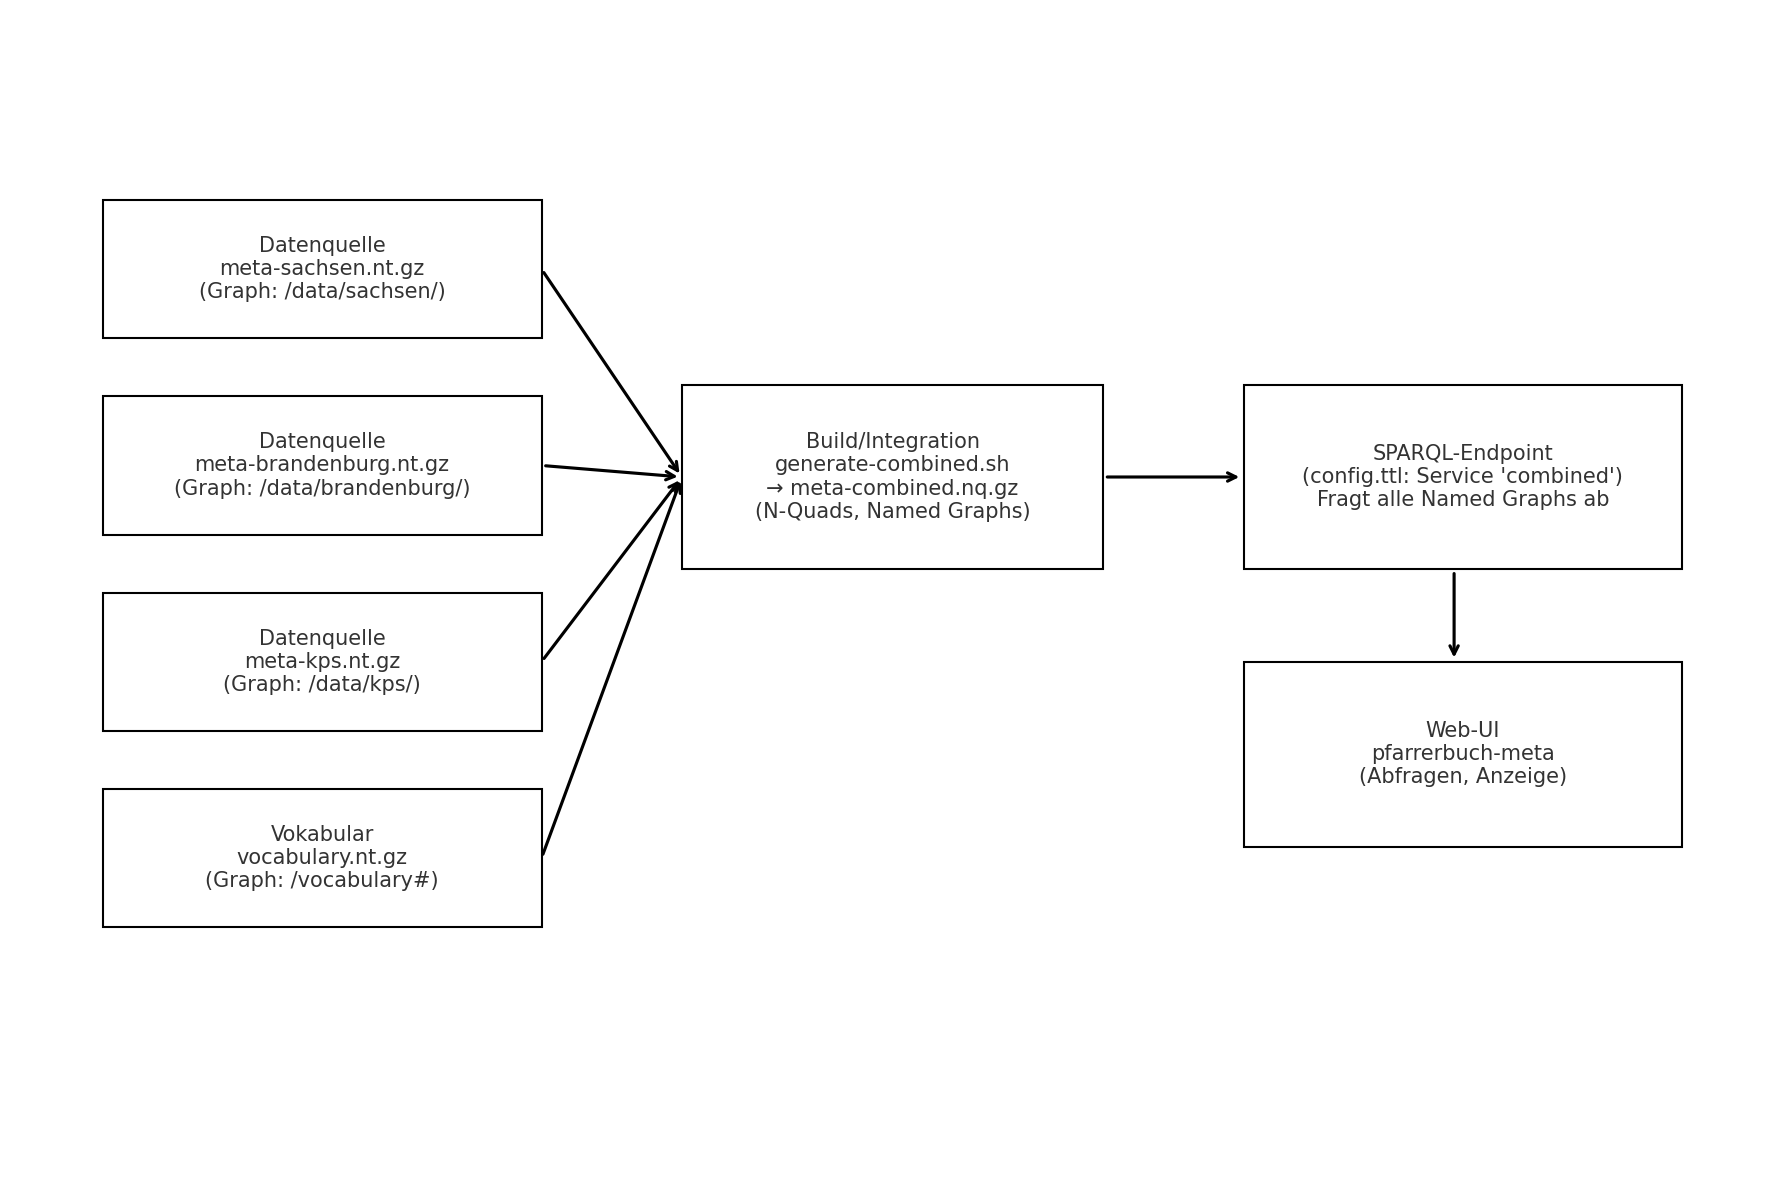
\includegraphics[width=\linewidth]{Abbildungen/Aufbau_Pfarrerdatenbank.jpg}
\caption{Architektur der Pfarrerdatenbank (Quellen $\rightarrow$ Build/Integration $\rightarrow$ kombinierter SPARQL-Dienst $\rightarrow$ Web-UI).}
\label{fig:pfarrer-architektur}
\end{figure}

\noindent Die Abbildung zeigt die vier Bausteine: (1) regionale N-Triples und Vokabular, (2) Skriptbasierter Merge nach N-Quads
(\texttt{meta-combined.nq.gz}) mit benannten Graphen, (3) SPARQL-Endpoint \emph{combined} aus \texttt{config.ttl}, (4) die Web-UI.

\subsection{SPARQL-Beispiele}
\noindent Präfixe (für alle Beispiele):
\begin{verbatim}
PREFIX pfb: http://meta-pfarrerbuch.evangelische-archive.de/vocabulary#

PREFIX rdf: http://www.w3.org/1999/02/22-rdf-syntax-ns#

PREFIX rdfs:http://www.w3.org/2000/01/rdf-schema#

PREFIX xsd: http://www.w3.org/2001/XMLSchema#

\end{verbatim}

\paragraph{(a) Anzahl Personen gesamt und pro Graph}
\begin{verbatim}
SELECT (COUNT(DISTINCT ?p) AS ?personenGesamt) WHERE {
?p rdf:type pfb:Person .
}

SELECT ?g (COUNT(DISTINCT ?p) AS ?anzahl) WHERE {
GRAPH ?g { ?p rdf:type pfb:Person . }
} GROUP BY ?g
\end{verbatim}

\paragraph{(b) Personen mit Name und Geburtsjahr}
\begin{verbatim}
SELECT ?p ?nach ?vor ?jahr WHERE {
?p rdf:type pfb:Person ;
pfb:nachname ?nach ;
pfb:vorname ?vor ;
pfb:hatLebensabschnitt ?la .
?la rdf:type pfb:Geburt .
OPTIONAL { ?la pfb:jahr ?jahr }
} LIMIT 50
\end{verbatim}

\paragraph{(c) Auf Sachsen eingrenzen (benannter Graph)}
\begin{verbatim}
SELECT ?p ?nach ?vor WHERE {
GRAPH http://meta-pfarrerbuch.evangelische-archive.de/data/graphs/sachsen
 {
?p rdf:type pfb:Person ;
pfb:nachname ?nach ;
pfb:vorname ?vor .
}
} LIMIT 50
\end{verbatim}

\paragraph{(d) Geburtsort (sofern vorhanden)}
\begin{verbatim}
SELECT ?p ?nach ?vor ?ort WHERE {
?p rdf:type pfb:Person ;
pfb:nachname ?nach ;
pfb:vorname ?vor ;
pfb:hatLebensabschnitt ?la .
?la rdf:type pfb:Geburt .
OPTIONAL { ?la pfb:hatOrt ?ort }
} LIMIT 50
\end{verbatim}

\subsection{Fazit}
Die Pfarrerdatenbank stellt einen integrierten RDF-Wissensgraph über mehrere Regionen bereit. Das eigene Vokabular und die klare Trennung per benannten Graphen ermöglichen sowohl aggregierte Queries als auch präzise Regionalsichten. Über den kombinierten SPARQL-Endpunkt versorgt die Web-UI Forschende und die interessierte Öffentlichkeit mit konsistenten, zitierfähigen Daten.








\section{Einführung in Large Language Models}
\label{sec:llm}

\subsection{Einordnung und Motivation}
Große Sprachmodelle (Large Language Models, LLMs) sind neuronale Netze, die auf umfangreichen Textkorpora mit einem Sprachmodellierungsziel vortrainiert werden und anschließend via Prompting, ggf.\ Feintuning und Ausrichtung (z.\,B.\ RLHF) eine breite Palette von Sprachaufgaben bearbeiten.\footnote{Ein einführender Überblick findet sich u.\,a.\ in \cite{campesatoLLMIntro}.} 
Zentraler Treiber ist die \emph{Transformer}-Architektur \cite{vaswani2017attention} kombiniert mit (i) Skalierung, (ii) In-Context-Lernen \cite{brown2020language,wei2022chain}, (iii) \emph{Tool-Use} \cite{yao2023react} und (iv) Instruction Tuning/RLHF \cite{ouyang2022training}. Dieses Kapitel bündelt die Grundlagen und verknüpft sie mit Sicherheit, Datenschutz und Retrieval \cite{abadi2016deep,carlini2021extracting,lewis2020rag}.

\subsection{Transformer‐Grundlagen}
Der Transformer ersetzt rekurrente/konvolutionale Netze durch \emph{Self-Attention}. Für Token-Repräsentationen $X$ werden \emph{Queries}, \emph{Keys}, \emph{Values} berechnet, und
\[
\mathrm{Attention}(Q,K,V)= \mathrm{softmax}\!\left(\frac{QK^\top}{\sqrt{d_k}}\right) V
\]
aggregiert kontextabhängig \cite{vaswani2017attention}. \emph{Multi-Head}-Attention modelliert verschiedene Relationen parallel; Positionsinformationen kommen über (gelernte) Encodings. Decoder-only-Modelle (GPT) modellieren $p(x_t\!\mid\!x_{<t})$ und sind Standard für generatives Prompting \cite{brown2020language}. Vortraining nutzt typischerweise \emph{Causal LM} auf großen, gefilterten Webkorpora.

\subsection{Dekodierung und Textqualität}
Greedy/Beam erzeugen oft wiederholungsreiche, „zu wahrscheinliche“ Texte; stochastische Verfahren wie \emph{Top-$k$}/\emph{Nucleus Sampling} erhöhen Varianz. Holtzman et\,al.\ zeigen \emph{Neural Text Degeneration} und empfehlen kalibriertes Sampling (\emph{nucleus}) sowie klare Stopkriterien \cite{holtzman2020curious}.

\subsection{Skalierung und In-Context-Lernen}
GPT-3 \cite{brown2020language} demonstriert starke Zero-/Few-Shot-Leistung rein per Prompting; Zugewinne steigen mit Modellgröße und Zahl der Demonstrationen. Nützliche Muster: Instruktions-Prompting, wenige prägnante Beispiele, explizite Formatvorgaben \cite{brown2020language,wei2022chain}.

\subsection{CoT und ReAct}
\emph{Chain-of-Thought} (CoT) ergänzt Beispiele um Zwischenschritte und verbessert mehrschrittiges Denken; Gewinne sind v.\,a.\ bei größeren Modellen ausgeprägt \cite{wei2022chain}. \emph{ReAct} verknüpft Denken und Handeln (Search/Lookup), reduziert Halluzinationen und erhöht Nachvollziehbarkeit \cite{yao2023react}. Beide sind relevant, wenn natürlichsprachliche Anweisungen in SPARQL-Strukturen zu überführen sind.

\subsection{Instruction Tuning und RLHF}
Instruction Tuning (SFT), Präferenzlernen und RL (PPO mit KL-Regularisierung) führen zu von Menschen bevorzugten Antworten; teils übertreffen kleinere, ausgerichtete Modelle große, nicht-ausgerichtete Baselines \cite{ouyang2022training}. Bias/Halluzination bleiben offene Punkte.

\subsection{Wissensintensive Aufgaben: RAG \& KG-QA}
\emph{Retrieval-Augmented Generation} trennt parametrisierte Weltkenntnis (LM) und nicht-parametrisches Wissen (Index) \cite{lewis2020rag}. Pipeline: Query $\rightarrow$ Retriever (BM25/DPR/ColBERT) $\rightarrow$ Evidenzaggregation $\rightarrow$ Generator. Vorteile: Aktualität, Attribution, weniger Halluzination. Für \emph{Knowledge Graph QA} koppeln Ansätze Retrieval/Reasoning mit SPARQL; LC-QuAD~2.0 liefert komplexe, mehrhopfige Fragen über Wikidata/DBpedia \cite{dubey2019lcquad2}.

\subsection{Strukturierte Ausgaben (SPARQL/JSON)}
LLMs sind „free-form“, viele Anwendungen verlangen \emph{strukturierte} Ausgaben. Optionen: (i) \emph{Constrained Decoding} mit Grammatik/Regex/JSON-Schema, (ii) \emph{Schema-Prompting} mit strikten Beispielen, (iii) \emph{RL} mit Schema-basiertem Reward \cite{cong2023schema}. Für diese Arbeit ist das entscheidend, um valide SPARQL-Updates zu erzeugen.

\subsection{Sicherheit, Datenschutz und verantwortungsvolle Nutzung}
Modelle können Trainingsfragmente (inkl.\ PII) memorisieren; Extraktion ist gezeigt \cite{carlini2021extracting}. Gegenmaßnahmen: Datenkurationshygiene, konservatives Dekodieren, Quellenbindung (RAG/Tool-Use) \cite{lewis2020rag,yao2023react}. \emph{Differential Privacy} (DP-SGD) begrenzt den Beitrag einzelner Beispiele formal, mit Genauigkeits-Trade-offs \cite{abadi2016deep}. In Deployments sind Logging-Policies, Datenminimierung und Transparenz zentral.

\subsection{Evaluierung}
Perplexity ist nur Vorindikator. Aufgabenmetriken (EM/F1/ROUGE/Accuracy) und menschliche Präferenzbewertungen sind komplementär \cite{ouyang2022training}. Für CoT/Tool-Use sollten auch \emph{Rationale}/Trajektorien bewertet werden (Korrektheit, Konsistenz, Zitierbarkeit).

\subsection{Grenzen und offene Herausforderungen}
\begin{itemize}
  \item \textbf{Effizienz}: Kontextlänge, $\mathcal{O}(n^2)$-Attention; Abhilfe durch Retrieval, Sparsity, Distillation.
  \item \textbf{Robustheit/Bias}: Datenkurationslücken; belastbare, reproduzierbare Evaluationen fehlen oft.
  \item \textbf{Erklärbarkeit}: Rationale sind nützlich, aber keine „wahren“ Gründe; Audit statt Interpretation.
\end{itemize}

\subsection{Praxisbausteine}
Für die in dieser Arbeit entwickelte Pipeline genügt ein schlanker Satz von Prompt-Bausteinen: Zero-/Few-Shot-Templates binden Rollenbeschreibungen und Formatvorgaben ein, ReAct-artige Sequenzen ergänzen optional Suche und Tool-Aufrufe, und strikte Schemaangaben erzwingen strukturierte Ausgaben (JSON/SPARQL) \cite{liu2023survey,yao2023react,cong2023schema}. Entscheidend ist weniger das konkrete Prompt-Layout als die Verzahnung mit nachgelagerten Guardrails (Validator, Explainability, Undo), die in den folgenden Kapiteln ausgearbeitet werden.

\subsection{Zusammenfassung}
LLMs kombinieren Transformernetzwerke, skalengetriebenes Vortraining und In-Context-Lernen zu universellen Sprachwerkzeugen. \emph{CoT} verbessert mehrschrittiges Denken, \emph{ReAct} verankert Antworten in externer Evidenz, \emph{RAG} ist zentral für wissensintensive Szenarien. Für diese Arbeit sind strukturierte Ausgaben (SPARQL), Guardrails und Datenschutzmaßnahmen (u.\,a.\ DP) entscheidend \cite{vaswani2017attention,brown2020language,wei2022chain,yao2023react,ouyang2022training,lewis2020rag,holtzman2020curious,abadi2016deep,carlini2021extracting,dubey2019lcquad2,cong2023schema}.









\section{Prompt-Programmierung und Few-Shot Learning}
\label{sec:prompting}

\subsection{Von \emph{Pre-Train, Fine-Tune} zu \emph{Pre-Train, Prompt, Predict}}
In der aktuellen Entwicklung der Sprachverarbeitung hat sich das Paradigma von rein aufgaben\-spezifischer Supervision hin zu vortrainierten Sprachmodellen (LMs) mit Aufgabenspezifikation über Prompts verschoben. Während klassische Systeme die bedingte Wahrscheinlichkeit \(P(y \mid x;\theta)\) direkt durch überwachten Lernens optimieren, modellieren Prompting-Methoden die Textwahrscheinlichkeit \(P(x;\theta)\) und reformulieren Aufgaben so, dass ein LM mit geeigneter Texteingabe (\emph{Prompt}) die gewünschte Ausgabe produziert \cite{liu2023survey}. Dieses \emph{Pre-Train, Prompt, Predict}-Denken bietet drei zentrale Vorteile: (i) Nutzung großskaliger Rohtexte für das Vortraining, (ii) wenige bis keine gelabelten Daten (\emph{few-/zero-shot}) durch geschickte Aufgabenformulierung, (iii) schnelle Adaptierbarkeit über Prompt- statt Objektiv-Engineering \cite{liu2023survey}.

\subsection{Bausteine des Promptings}
\textbf{Template-Engineering:} Formen wie \emph{Prefix}-Prompts (autoregressiv), \emph{Cloze}-Prompts (maskiert) oder Vorlagen für Mehrfacheingaben; Design manuell oder automatisiert \cite{liu2023survey}.\\
\textbf{Answer-Engineering:} Antwortraum gezielt einschränken (Labelwörter/Verbalizer vs.\ freie Generierung); auch hier manuell, heuristisch oder kontinuierlich optimiert \cite{liu2023survey}.\\
\textbf{Kontext \& Multiprompts:} Prompt-Ensembling (Mehrheitsvotum/Distillation) und \emph{In-Context}-Demonstrationen (Auswahl/Reihenfolge/Retrieval) stabilisieren; Komposition/Dekomposition macht Aufgabenstruktur explizit \cite{liu2023survey}.

\subsection{Trainingsstrategien im Prompting-Spektrum}
Ohne LM-Updates (\emph{tuning-frei}) ist Prompting effizient, aber prompt-sensitiv. Alternativen: \emph{Prompt-Tuning} (nur Prompt-Parameter), klassisches Feintuning mit fixem Prompt oder gemeinsame Optimierung (Prompt+LM) mit höherem Aufwand, aber mehr Kapazität \cite{liu2023survey}.

\subsection{Reasoning-Prompts: CoT, Self-Consistency, Kalibrierung}
\textbf{Chain-of-Thought (CoT):} Few-Shot-Beispiele inkl.\ Zwischenschritte (\emph{Rationale}) verbessern mehrschrittiges Denken, v.\,a.\ bei größeren Modellen \cite{wei2022cot}.\\
\textbf{Self-Consistency:} Statt einer CoT-Antwort mehrere Denkpfade sampeln und die konsistenteste Endlösung wählen; wenige Stichproben (5–10) genügen oft \cite{wang2022selfconsistency}.\\
\textbf{Kontextuelle Kalibrierung:} Korrigiert Antworttendenzen (z.\,B.\ Reihenfolge-/Common-Token-Bias) durch Vorab-Schätzung auf inhaltsfreien Inputs; senkt Varianz ohne Zusatzdaten \cite{zhao2021calibrate}.

\subsection{KGQA \& Text-zu-SPARQL}
Für Wissensgraph-Fragen ist \emph{Text-zu-SPARQL} robuster als Freitext: NL $\rightarrow$ SPARQL, Ausführung liefert belastbare Ergebnisse. Effektiv sind (i) T-Box- und A-Box-Nutzung, (ii) gezielte \emph{Fragmentierung} des relevanten Graphausschnitts, (iii) Generierung mehrerer Query-Varianten mit Auswahl per Ausführungserfolg \cite{avila2024autokgqagpt}. Praktische Leitlinien: Präfixe/Namespaces sichern, optionale Properties als \texttt{OPTIONAL}, String-Filter konsistent (Regex, \texttt{i}-Flag) \cite{avila2024autokgqagpt}.

\subsection{Von Prompt-Ketten zu Pipelines: DSPy}
\emph{DSPy} beschreibt LM-Schritte deklarativ (\emph{Signaturen, Module}) und kompiliert automatisch zu hochwertigen Prompt-/Finetuning-Strategien. Teleprompter bootstrappen Demonstrationen, wählen Hyperparameter und können feintunen oder ensemblen \cite{khattab2023dspy}. Vorteil: weniger fragile Strings, mehr reproduzierbare, selbstverbessernde Pipelines—nützlich für Multi-Hop-Retrieval, KGQA oder Agent-Loops.

\subsection{Offene Punkte und Best Practices}
\textbf{Offene Punkte:} Prompt-Transfer über Modellfamilien, Kosten von CoT/Ensembles, Bias/Format-Effekte trotz Kalibrierung, strukturierte Ausgaben für Tabellen/Graphen \cite{liu2023survey,zhao2021calibrate}.\\
\textbf{Konkret umsetzbar:}
\begin{enumerate}
  \item Aufgabe präzisieren $\rightarrow$ passende Promptform (Prefix/Cloze) \& kleiner Antwortraum.
  \item Stabilität: \emph{In-Context}-Demonstrationen + kontextuelle Kalibrierung \cite{zhao2021calibrate}.
  \item Denkaufgaben: \emph{CoT} einschalten; bei Bedarf \emph{Self-Consistency} (5–10 Pfade) \cite{wei2022cot,wang2022selfconsistency}.
  \item Wissensfragen: strukturierte Exekution (SPARQL) statt Freitext; KG-Fragmentierung strikt halten \cite{avila2024autokgqagpt}.
  \item Pipelines: deklarativ mit \emph{DSPy} bauen; Compiler Demonstrationen/Hyperparameter wählen lassen \cite{khattab2023dspy}.
\end{enumerate}

\subsection{Fazit}
Prompting verlagert den Schwerpunkt von datenintensiver Supervision zu geschickter Aufgabenformulierung. Mit Template-/Answer-Engineering, CoT+Self-Consistency und Kalibrierung entstehen robuste Systeme; für wissensintensive Domänen ist \emph{Text-zu-SPARQL} eine präzise, halluzinationsarme Strategie. Deklarative Pipelines (DSPy) erhöhen Reproduzierbarkeit und Wartbarkeit \cite{liu2023survey,wei2022cot,wang2022selfconsistency,zhao2021calibrate,avila2024autokgqagpt,khattab2023dspy}.






\section{Query-Validierung und Explainability im RDF/SPARQL-Stack}
\label{chap:Query-validation-explainability}

\subsection{Motivation}
RDF/RDFS/OWL definieren primär \emph{Struktur}. Für belastbare Datenprodukte braucht es zusätzlich (i) \textbf{Validierung} gegen modellierte Erwartungen, (ii) \textbf{Erklärbarkeit} (Provenienz \& Why-Not), (iii) \textbf{beherrschte OPTIONAL}-Nutzung. Wir kombinieren dafür: SPIN für modellnahe Validierung/Regeln \cite{spin-w3c}, schwach gut konzipiertes (wwd) SPARQL für sichere \texttt{OPTIONAL}s \cite{kaminski-kostylev-beyond-well-designed} und Provenienz-Halbringe als algebraisches Fundament \cite{green-provenance-semirings,herschel-why-why-not,herschel-survey}.

\subsection{Validierung mit SPIN}
\textbf{SPIN} (\emph{SPARQL Inferencing Notation}) repräsentiert SPARQL als RDF und verknüpft Abfragen direkt mit Klassen:
\begin{itemize}
  \item \texttt{spin:constraint} (ASK/CONSTRUCT): Bedingungen, die Instanzen erfüllen müssen.
  \item \texttt{spin:rule}: Inferenz via CONSTRUCT/UPDATE.
  \item \texttt{spin:constructor}: Initialwerte beim Anlegen neuer Instanzen.
\end{itemize}
Abfragen laufen im Klassenkontext mit vorgebundener Variable \texttt{?this}; Vererbung folgt \texttt{rdfs:subClassOf}. \texttt{spin:thisUnbound=true} erlaubt Optimierungen \cite{spin-w3c}. \emph{CONSTRUCT}-Constraints können \texttt{spin:ConstraintViolation} erzeugen (mit \texttt{spin:fix}-Hinweisen).

\paragraph{Minimalbeispiel.}
\begin{lstlisting}[language=turtle,basicstyle=\ttfamily\small]
@prefix ex: <http://example.org/> .
@prefix rdfs: <http://www.w3.org/2000/01/rdf-schema#> .
@prefix spin: <http://spinrdf.org/spin#> .
@prefix sp: <http://spinrdf.org/sp#> .

ex:Square a rdfs:Class ;
  spin:constraint [ a sp:Ask ;
    sp:text """ASK { ?this ex:width ?w ; ex:height ?h .
                     FILTER(?w != ?h) }""" ] .
\end{lstlisting}

\paragraph{Praxisleitfaden.}
(1) Prüfungen als \texttt{ASK} (schnell), Violations optional via \texttt{CONSTRUCT}. (2) Regeln/Constraints \emph{klassenlokal} und granular halten. (3) UPDATE-Regeln begrenzen (Iterationslimit/Reihenfolge), um Loops zu vermeiden.

\subsection{Explainability: Provenienz \& Why-Not}
Mit \emph{K-Relationen} werden Tupel durch Elemente eines kommutativen Halbrings annotiert; die relationale Algebra (bzw.\ Datalog) hebt sich homomorph auf Annotationen \cite{green-provenance-semirings}. Ergebnis:
\begin{itemize}
  \item \textbf{How-Provenienz}: Polynome kodieren, \emph{wie} Quellen kombiniert wurden.
  \item \textbf{Why-Provenienz}: Zeugen(-basen) zeigen, \emph{welche} Quelltupel genügen.
  \item \textbf{Where-Provenienz}: positionale Herkunft (Zell-/Attributebene).
\end{itemize}
\textbf{Why-Not} (fehlende Antworten) lässt sich (i) \emph{instanzbasiert} (abduktiv: minimale Datenupdates, die die Antwort erzeugen) oder (ii) \emph{abfragebasiert} (operatorzentriert: welcher Operator/Filter schneidet ab) erklären; hybride Ansätze verbinden beides \cite{herschel-why-why-not,herschel-survey}. Operativ empfiehlt sich: Top-Level-Filter und verworfene Muster protokollieren; Visualisierung als kompakte Summaries statt roher Graphen.

\subsection{OPTIONAL richtig einsetzen: wwd-SPARQL}
\texttt{OPTIONAL} ermöglicht Teilantworten, macht generelle Auswertung aber schwer. Das \emph{gut konzipierte} Fragment (wd) deckt die Praxis nur teilweise; \textbf{wwd} erweitert wd und behält \emph{coNP}-Auswertbarkeit \cite{kaminski-kostylev-beyond-well-designed}. Kernregeln:
\begin{itemize}
  \item Variablen von rechten \texttt{OPT}-Seiten dürfen außerhalb nur auftreten, wenn ihr Auftreten \emph{dominiert} (links).
  \item FILTER, die solche Variablen referenzieren, \emph{nur} auf oberster Ebene.
  \item Normalformen \emph{OPT-FILTER-Normalform} (OF) und \emph{Constraint Pattern Trees} (CPT) machen Prioritäten explizit.
\end{itemize}
\textbf{Best Practices:} Links-assoziieren \((P_1\ \mathrm{OPT}\ P_2)\ \mathrm{OPT}\ P_3\) statt \(P_1\ \mathrm{OPT}\ (P_2\ \mathrm{OPT}\ P_3)\); tiefe \texttt{OPT}-Nester vermeiden; FILTER für rechte \texttt{OPT}-Variablen nur top-level.

\subsection{Mini-Playbook}
\begin{enumerate}
  \item \textbf{Modellieren}: RDFS/OWL-Schema + SPIN-\texttt{constraint}s; optionale SPIN-\texttt{rule}s für Anreicherung.
  \item \textbf{Früh validieren}: Formulare/ETL mit \texttt{ASK}-Constraints; Violations als \texttt{ConstraintViolation} mit \texttt{spin:fix}.
  \item \textbf{Abfragen robust bauen}: wwd-Form als Ziel; OF/CPT prüfen.
  \item \textbf{Erklärbarkeit sichern}: How/Why-Provenienz; Why-Not-Logs (Top-Level-Filter, verworfene Muster).
  \item \textbf{Governance}: dereferenzierbare URIs für SPIN-Bibliotheken; Regeliteration begrenzen.
\end{enumerate}

\subsection{Grenzen und Ausblick}
SPIN bringt Validierung \emph{ins Modell}, verlangt aber Disziplin (Terminierung/Updates). Wwd hält \texttt{OPTIONAL} praktikabel, OF/CPT kann jedoch wachsen. Provenienz skaliert fachlich, nicht beliebig speicherseitig; visuelle Summarisierung bleibt zentral \cite{herschel-survey}. 






\section{Datenschutz und Anonymisierung in SPARQL-Operationen}
\label{sec:privacy}

Dieses Kapitel bündelt Rechtsgrundlagen, Angreifermodelle und technische Maßnahmen für Datenschutz in SPARQL-basierten Systemen (RDF-Speicher, Linked-Data-APIs, Query-Logs). Im Fokus: Zugriffskontrolle, Pseudonymisierung/Anonymisierung von RDF-Graphen, differentielle Privatsphäre (für Antworten \emph{und} Logs), k-Anonymität via Mikroaggregation sowie Betriebsleitlinien (Fuseki/Jena) entlang der W3C \emph{Data on the Web Best Practices} und des \emph{Data Privacy Vocabulary}.

\subsection{Grundlagen: Rechtsrahmen und Begriffe}
\textbf{Rechtsmaßstab.} Nach EU-DSGVO ist \emph{Anonymisierung} irreversibel; \emph{Pseudonymisierung} reduziert Identifizierbarkeit, bleibt aber personenbezogen. Der Art.-29-APK prüft \emph{Singling-out}, \emph{Linkability}, \emph{Inference} \cite{Art29WPAnonymisation,enisa2019pseudonymisation}. \\
\textbf{Privacy-by-Design.} W3C \emph{Privacy Principles} fordern Zweckbindung, Datenminimierung, Sicherheit, Transparenz/Wahlmöglichkeiten, Verantwortlichkeit \cite{W3CPrivacyPrinciples}. DPV beschreibt Zwecke, Rechtsgrundlagen, Empfänger, Speicherfristen als maschinenlesbare Metadaten \cite{W3CDPV}; Veröffentlichungen folgen W3C DWBP (Provenienz, Versionierung, Mehrformate, Feedback) \cite{W3CDWBP}.

\subsection{Angreifermodelle und Schutzziele}
\textbf{Angreifer:} (i) passiv (öffentl.\ Endpunkte/Dumps), (ii) aktiv (Injektion/Sybil/Poisoning), (iii) Verknüpfer (externe Linkage). \textbf{Schutzziele:} (a) Re-Identifikation verhindern, (b) Linkage-Risiko senken, (c) Inferenz über sensible Attribute begrenzen, (d) Verfügbarkeit/Nutzwert erhalten.

\subsection{Zugriffskontrolle als Grundschutz (AuthN/AuthZ)}
\textbf{Serverseitig.} Apache Fuseki: HTTPS, Basic/Digest (nur über TLS), ACLs auf Server-/Datensatz-/Endpunkt- und (read-only) Graph-Ebene; Steuerung von Default-/Union-Graph \cite{FusekiAccess}. \\
\textbf{In-Graph-Policies.} \emph{Jena Permissions} erzwingt CRUD-Entscheidungen pro Principal (Graph, optional Triple) via \texttt{SecurityEvaluator}, inkl.\ Caching \cite{JenaPermissions}. \\
\textbf{Praxis:} TLS mit vertrauenswürdigen Zertifikaten, Least-Privilege-ACLs, Trennung \emph{Rohdaten} vs.\ \emph{publike Derivate}, Audit-Logging.

\subsection{Pseudonymisierung vs.\ Anonymisierung}
\textbf{Pseudonymisierung.} Reines Tokenisieren/Hashen von IDs/Query-Tokens ist anfällig (Frequenz/Kontext); robust: Salt, Schlüsselrotation, Kontext-Verdrillung. \\
\textbf{Anonymisierung.} Für Veröffentlichungen sind formale Verfahren nötig: differentielle Privatsphäre (DP) oder strikte k-Anonymität (mit bekannten Grenzen).

\subsection{Anonymisierung von RDF-Graphen}
\textbf{Risiken.} RDF ist über Identifikatoren und Topologie linkbar; Linkage nutzt Muster, Attributdomänen, externe Datensätze \cite{delanaux-linkage,logical-foundations-lda}. \\
\textbf{Optionen.} (i) Zufalls-/generaliserte IRIs für lokale Ressourcen, (ii) Attribut-Binning/Hierarchien, (iii) Topologie-Vergröberung (Entität$\rightarrow$Typ/Superklasse), (iv) strikte Provenienz (PROV-O) der Transformationen.

\subsection{Differential Privacy (DP) für SPARQL}
\textbf{Definition.} Ein Mechanismus $A$ ist $\varepsilon$-DP, wenn für benachbarte Datensätze $D,D'$ und Ausgaben $O$ gilt:
\[
  \Pr\!\big[A(D)=O\big] \le e^{\varepsilon}\,\Pr\!\big[A(D')=O\big].
\]

Schwächungen: $(\varepsilon,\delta)$-DP und \emph{probabilistic DP} (mit Wkt.\ $\ge1-\delta$) \cite{GoetzZealous}. \\
\textbf{SPARQL-spezifisch.} Direkt anwendbar auf monotone Aggregationen (\texttt{COUNT}/\texttt{SUM} mit begrenzter Sensitivität); frei kombinierte \texttt{OPTIONAL}/\texttt{FILTER}-Muster erhöhen Sensitivität und Analyseaufwand \cite{builaranda-dp-sparql}. \\
\textbf{Praxisleitfaden.} (a) Aggregations-\emph{Fragment} mit statischer Kardinalitätsgrenze, (b) \emph{Per-User Contribution Capping} ($\le m$ Beiträge/Nutzer), (c) Sitzungsbudget $\varepsilon$ (Komposition beachten), (d) Post-Processing (Negativwerte truncaten, Seltenes filtern). \\
\textbf{Mechaniken am Endpunkt.} (1) Antwort-Perturbation (Laplace/Geometrisch) mit Konfidenzintervallen; (2) Schema-Perturbation (verrauschte Histogramme); (3) Query Auditing/Refusal bei zu hoher Sensitivität.

\subsection{Logs \& Nutzungsspuren: ZEALOUS, Mikroaggregation, Streaming}
\textbf{ZEALOUS (häufige Items).} Mittelweg zwischen strikter DP (oft zu restriktiv) und k-Anonymität (angreifbar): Beiträge pro Nutzer auf $m$ deckeln, Vorfilter $\tau$, Laplace-Rauschen, Nachfilter $\tau'$, nur verrauschte Top-Items veröffentlichen $\Rightarrow$ $(\varepsilon,\delta)$-\emph{probabilistic DP}/Ununterscheidbarkeit \cite{GoetzZealous}. \emph{Parameter:} fixiere $\delta$ (z.\,B.\ 0{,}001), wähle $\varepsilon\in[0{,}5,2]$, setze $\tau=\lceil2m/\varepsilon\rceil$, wähle $m$ unterhalb des Durchschnitts. \emph{Nutzwert:} Recall der Top-$J$ und L1/KL-Abstand. \\
\textbf{k-Anonymität via Mikroaggregation (User-Level).} Nutzer-Query-Bäume clustern (Zeit, Rang, Domain-Ähnlichkeit, Edit-/Hausdorff-Distanzen), Cluster-Schwerpunkt ersetzt Individualdaten $\Rightarrow$ Re-Identifikation $\le 1/k$ bei kontrolliertem Informationsverlust \cite{NavarroUserKAnon}. Grenzen: syntaktisch, gegen aktive Angriffe verwundbar. \\
\textbf{Online-Streaming.} Threshold-Kryptografie/Secret-Sharing: Rekonstruktion erst ab Schwellwert $t$ verschiedener Nutzer; alternativ Sitzungs-Splitting nach Interessensdomänen \cite{AdarQueryLogs}.

\subsection{Betriebsarchitektur für SPARQL mit Datenschutz}
\label{sec:privacy-governance}
\textbf{Schichten.} (1) \emph{Ingest/Private Zone}: Rohdaten/Logs, strenge ACLs (Fuseki), Jena Permissions. (2) \emph{Anonymisierungs-Layer}: DP-Aggregationen, ZEALOUS für häufige Items, mikroaggregierte Nutzeransichten (stärkere Policies). (3) \emph{Publikations-Zone}: read-only Datensätze, TLS, AuthN, Graph-ACLs; DCAT/DPV/PROV-O; Bulk-Dumps + API. \\
\textbf{Rate-Limit/Budget.} Pro Principal: Throttling, Captcha/Bot-Schutz, DP-Budget $\varepsilon$; Ablehnung hochsensitiver Anfragen. \\
\textbf{Versionierung/Provenienz.} Veröffentlichungen dokumentieren ($\varepsilon,\delta,m,\tau,\tau'$), Datenbasis (Zeit/Scope), Qualität, Lizenz; persistente URIs für „neueste“ vs.\ datierte Version (Memento) \cite{W3CDWBP}.

\subsection{Leitlinien \& Checkliste}
\begin{itemize}
  \item \textbf{Minimalprinzip:} so grob wie möglich, so fein wie nötig.
  \item \textbf{SPARQL-Fragment:} nur Aggregations-Untermenge mit begrenzter Sensitivität; Volltext nur auf Whitelist-Feldern.
  \item \textbf{DP für Aggregation:} Rauschen + Budget + per-user Capping.
  \item \textbf{Logs:} ZEALOUS für Trends; Mikroaggregation für nutzerzentrierte Analysen.
  \item \textbf{Betrieb:} TLS, AuthN, Graph/Triple-Policies, Audit; Rate-Limits/Retry-Delays.
  \item \textbf{Publikation:} DCAT/DPV/PROV-Metadaten, Lizenz, Version, Bulk+API, Feedbackkanal.
\end{itemize}

\subsection{Grenzen und Forschungslücken}
DP für allgemeines SPARQL (OPTIONAL, Rekursion, CONSTRUCT) bleibt offen; robuste RDF-Anonymisierung gegen starke Linkage-Gegner ist schwierig. Semantische Ähnlichkeiten statt reiner Edit-Distanzen könnten Mikroaggregation verbessern—mit erweitertem Angriffsraum. Praktisch bewährt sich die Kombination aus starkem Grundschutz (AuthN/Z), restriktivem SPARQL-Fragment, DP-Aggregationen und anonymisierten Veröffentlichungen.

\medskip
\noindent\textbf{Kernaussage.} K-Anonymität allein genügt nicht; strikte $\varepsilon$-DP ist oft zu restriktiv. In der Praxis trägt ein \emph{Policy+Mechanism}-Ansatz: starke Zugriffskontrolle, formal begründete Anonymisierung (ZEALOUS/DP) für häufige Items und—wo nötig—k-anonyme Nutzerprofile via Mikroaggregation, flankiert von sauberer Publikations-Governance (W3C-BPs, DPV, PROV).












\chapter{Verwandte Arbeiten}
\label{sec:related-work}

Dieses Kapitel ordnet unseren Beitrag entlang von fünf Strängen ein: (i) \emph{NL{\textrightarrow}SPARQL \& KGQA}, (ii) \emph{visuelle Query-Builder}, (iii) \emph{Anonymisierung \& Differential Privacy für RDF/SPARQL}, (iv) \emph{Zugriffskontrolle für RDF \& Linked Data}, und (v) \emph{Governance-Vokabulare (DPV)}. Quer dazu positionieren wir unsere \emph{Praxislösung} (Kap.~\ref{sec:implementierung}) mit Ontologie-only Prompting, Preview{\(\rightarrow\)}Execute-Guardrails, Undo, pseudonymisierten Logs und SHACL-/DPV-basierten Governance-Artefakten.

\subsection{NL{\textrightarrow}SPARQL und Fragebeantwortung auf Wissensgraphen}
Frühe neuronale Arbeiten zu \emph{NL{\textrightarrow}SPARQL} zeigen die Machbarkeit von Sequenz-zu-Sequenz-Übersetzungen \cite{yin-nmt-sparql}. LC-QuAD~2.0 etabliert komplexe Benchmarks (Wikidata/DBpedia) und fordert Generalisierung/Komposition \cite{lcquad2}. Zeitnahe Ansätze koppeln LLMs mit KG-Awareness, Retrieval und Strukturinduktion \cite{avila-kgqa-llm,pramanik-uniqorn}.

\textit{Bezug zu unserer Arbeit.} Während der Großteil der Literatur auf \textbf{SELECT/KGQA} zielt, setzt unser System explizit auf \textbf{Änderungsoperationen} (\texttt{INSERT}/\texttt{DELETE}/\texttt{DELETE/INSERT}) und bindet diese in einen \textbf{zweistufigen} Workflow ein (Preview mit Validation/Explain {\(\rightarrow\)} tokenpflichtige Execute-Phase) inkl.\ deterministischem \textbf{Undo} (Kap.~\ref{sec:konzeption}, \ref{sec:implementierung}). Anders als schema-agnostische Übersetzer geben wir dem LLM nur die \textbf{Ontologie (T-Box)} statt Instanzdaten (\emph{Privacy-by-Design}) und prüfen vor Ausführung \emph{ontologiekonforme} Tripel (Validator-Service, Explainability-Panel; Kap.~\ref{sec:evaluation}).

\subsection{Visuelle SPARQL-Builder und Exploration}
Die YASGUI-Familie ist De-facto-Standard für Editor/Endpoint-Interaktion/Shareability \cite{yasgui}. Domänenspezifische Builder wie \emph{RDF Explorer} \cite{vargas-rdf-explorer} oder der \emph{Wikidata Query Builder} senken Einstiegshürden; Kuric~et~al.\ diskutieren Usability-Herausforderungen bei Laien \cite{kuric-usability}.

\textit{Bezug zu unserer Arbeit.} Unser UI kombiniert YASGUI-artige Editor-Erfahrung mit \textbf{Guided Patterns}, \textbf{Preview/Explain}, \textbf{Ablauf-Token} (Countdown) und \textbf{Undo}-Buttons sowie einem \textbf{Logs-Panel} (pseudonymisiert) und \textbf{PerfPanel} (p50/p95/max; Kap.~\ref{sec:implementierung}). Damit adressieren wir die in \cite{kuric-usability} beschriebenen Einstiegshürden durch unmittelbare Rückmeldungen (Validation/Explain) und sichere Ausführung (Token-Gate). Die Evaluation (Kap.~\ref{sec:evaluation}) zeigt, dass Nutzer:innen mit TODO-Hinweisen/Platzhaltern im Editor umgehen und Korrekturen zielgerichtet vornehmen.

\subsection{Anonymisierung, Linkage-Robustheit und Differential Privacy}
Formale Garantien sind im Linked-Data-Kontext schwieriger als in Tabellenmodellen: logikbasierte Arbeiten beschreiben Voraussetzungen/Grenzen von RDF-Anonymisierung \cite{logical-foundations-lda}; Delanaux~et~al.\ adressieren strukturbezogene Linkage-Robustheit \cite{delanaux-linkage}. Für SPARQL diskutiert Buil-Aranda DP-Strategien (z.\,B.\ \emph{noisy aggregates}, Budgete) \cite{builaranda-dp-sparql}.

\textit{Bezug zu unserer Arbeit.} Produktiv setzen wir \textbf{deterministische Pseudonymisierung} für Logs ein (Namen/URIs {\(\rightarrow\)} Token), während die \textbf{LLM-Pipeline Ontologie-only} bleibt (keine A-Box im Prompt). \textbf{DP- und ZEALOUS-Mechanismen} werden als \emph{Erweiterungspunkte} architektonisch vorbereitet (Kap.~\ref{sec:privacy}, \ref{sec:privacy-governance}); die Betriebsleitlinien empfehlen ein \emph{restriktives Aggregations-Fragment} und Budgetierung. Damit positioniert sich unser System zwischen praktischer Einsetzbarkeit (Pseudonymisierung, Zugriffskontrolle) und forschungsnahen, optionalen DP-Modulen.

\subsection{Zugriffskontrolle für RDF und Linked Data}
Kirrane~et~al.\ systematisieren Modelle (MAC, DAC, RBAC), moderne ABAC/CBAC-Varianten und RDF/LD-spezifische Durchsetzung \& Standards \cite{kirrane-ac-survey}. Diskutiert werden View-basierte Kontrollen (VBAC), Delegation/Widerruf, XACML/ODRL, WebID/WAC und Policy-Engines (z.\,B.\ SHI3LD) mit ASK/Rewrites \cite{kirrane-ac-survey}.

\textit{Bezug zu unserer Arbeit.} Wir trennen \textbf{Produktionsgraphen} von einem \textbf{Changes-Graph} (<\texttt{urn:nl2sparql:changes}>) für Undo/Revisionen und erzwingen \textbf{Pre-Enforcement} durch Validation/Explain + Token (Kap.~\ref{sec:implementierung}). Das Backend implementiert \textbf{AuthN} (API-Key) und \textbf{Rate-Limits}; ABAC/VBAC-Policies und \textbf{SHACL-Prechecks} sind im Design verankert (Meta-Policies, \emph{deny-overrides}) und auf Fuseki/Jena-Mechanismen (ACLs, Jena Permissions) abbildbar (Kap.~\ref{sec:privacy-governance}). Damit schlagen wir eine Brücke zwischen Literaturmodellen und einer leichtgewichtigen, praktischen Durchsetzung in Editier-Workflows.

\subsection{Governance mit dem Data Privacy Vocabulary (DPV)}
DPV (W3C DPVCG) beschreibt Zwecke, Rechtsgrundlagen, Rollen, Datenkategorien, Bedingungen, Maßnahmen und Rechte; v2.0 erweitert dies um TECH/AI/LEGAL-Erweiterungen \cite{dpv2024w3c}.

\textit{Bezug zu unserer Arbeit.} Jede NL{\(\rightarrow\)}SPARQL-Operation wird als \textbf{Governance-Akte} gedacht: Wir modellieren sie (konzeptionell) als \texttt{dpv:Process} mit \texttt{hasPurpose}, \texttt{has(LegalBasis|PersonalData|Processing)} und \texttt{has(Technical|Organisational)Measure} und prüfen diese via \textbf{SHACL-Prechecks} \emph{vor} Ausführung (Kap.~\ref{sec:konzeption}, \ref{sec:privacy-governance}). In der UI werden Governance-Artefakte (z.\,B.\ Zweck/Legal-Basis-Auswahl) als \emph{Guided Patterns} sichtbar; unser Logger verknüpft Explain/Undo mit pseudonymisierten Inhalten (Kap.~\ref{sec:implementierung}).

\paragraph{Einordnung unseres Beitrags.}
\begin{enumerate}
  \item \textbf{Von Query-Synthese zu \emph{sicherer} Datenänderung:} Über reine SELECT/KGQA hinaus generieren wir \texttt{INSERT}/\texttt{DELETE}/\texttt{UPDATE} und erzwingen einen Preview{\(\rightarrow\)}Execute-Flow mit Token und Undo.
  \item \textbf{Privacy-by-Design:} Ontologie-only Prompting, pseudonymisierte Logs, Changes-Graph und (optionale) DP/ZEALOUS-Erweiterungen.
  \item \textbf{Policy-First:} SHACL-gestützte Pre-Enforcement-Prüfungen und DPV-Integration in den Prozessfluss statt reiner „Best-Effort“-Ausführung.
  \item \textbf{Usability \& Monitoring:} Guided Editor, Explainability, Undo, sowie Metriken (p50/p95/max) für Endpunkt- und LLM-Latenzen.
\end{enumerate}
In Summe positioniert sich unsere Arbeit zwischen den Linien NL{\(\rightarrow\)}SPARQL/KGQA, Policy/Access-Control und Privacy-Mechanismen als \emph{praktikable} Brücke: ein LLM-gestützter, revisionssicherer Editor für RDF-Änderungen mit Governance-„First“-Prinzip.





\chapter{Anforderungsanalyse und Konzeption}
\label{sec:konzeption}

Dieses Kapitel konkretisiert die in Kapitel~\ref{sec:Einleitung} formulierte Zielsetzung und führt die Brücke zum Implementierungsteil. Auf Basis des Semantic-Web- und LLM-Hintergrunds aus Kapitel~\ref{sec:theorie} sowie der Domänenanalyse (Kapitel~\ref{sec:Pfarrerdatenbank}) werden Anforderungen strukturiert, in eine modulare Architektur überführt und mit passender Benutzerführung hinterlegt.

\section{Zielsetzung und Scope}
Ziel ist eine \textbf{assistierte, nachvollziehbare Bearbeitung} RDF-basierter Wissensbestände. Natürlichsprachliche Änderungswünsche werden in SPARQL-Updates (INSERT/DELETE/UPDATE) überführt, validiert, erklärt, zweistufig bestätigt und revisionssicher protokolliert. Der LLM-Kontext enthält ausschließlich die Ontologie (T-Box); Instanzdaten bleiben im Triple-Store. Ausgenommen sind kollaboratives Echtzeit-Editing, großskalige Cluster-Deployments und komplexe Migrationsszenarien. Diese bleiben über definierte Erweiterungspunkte adressierbar.

\section{Stakeholder und Nutzungskontext}
\begin{description}
  \item[Domänenexperten/-expertinnen] (z.\,B.\ Archivpersonal) formulieren Änderungswünsche in natürlicher Sprache und prüfen Vorschau/Erklärungen, bevor sie ausführen.
  \item[Datenkurator:innen] überwachen Änderungshistorie und Kennzahlen, nutzen Undo und bewerten Datenschutzmaßnahmen.
  \item[Systemadministration] betreibt Backend und Fuseki, pflegt Konfigurationen (API-Key, Fuseki-Zugang, Logging) und kontrolliert Datenschutz-Policies.
\end{description}

\paragraph{Beispielszenario.} Eine Archivar:in erfasst eine Korrektur („Ändere den Nachnamen von Pfarrer Martin Müller in Meier“). Das System generiert einen Vorschlag, erklärt die Auswirkungen, fordert eine Bestätigung mittels Token und protokolliert Ergebnis sowie Undo-Information. Im Fehlerfall kann ein/e Kurator:in die Änderung zurücknehmen und die Ursachen analysieren.

\section{Funktionale Anforderungen}

\subsection*{F1~–~NL-gestützte Datenänderung}
Unterstützung für Einfügen, Ändern und Löschen von Tripeln über natürlichen Text. Die semantische Abbildung erfolgt gegen die bereitgestellte Ontologie; siehe Services in Abschnitt~\ref{subsec:arch-backend}.

\subsection*{F2~–~Vorschau und Erklärbarkeit}
Vor Ausführung liefert das System eine Preview mit (i) Schema-Validierung (Klassen, Properties, Präfixe), (ii) verbaler Kurzbeschreibung und (iii) strukturiertem Diff. Dies schlägt sich in den Endpunkten \texttt{/nl2sparql/preview} und \texttt{/nl2sparql/explain} nieder.

\subsection*{F3~–~Zweistufige Bestätigung}
Preview erzeugt ein \texttt{confirm\_token} mit TTL; Execute verbraucht dieses Token und führt die Änderung atomar aus. Der Flow korrespondiert mit den Guardrails in der UI und den Security-Hooks im Backend.

\subsection*{F4~–~Ontologie-only im LLM}
Der Prompt-Generator (vgl.\ Kapitel~\ref{sec:prompting}) stellt dem LLM nur Klassen und Properties bereit. Instanzdaten werden nicht externalisiert (Privacy-by-Design).

\subsection*{F5~–~Datenschutzmaßnahmen}
\begin{itemize}
  \item \textbf{NL-Anonymisierung:} Pre-Processing maskiert sensible Personen-/Ortsnamen (Vorname/Nachname/Gemeinde) vor dem LLM-Aufruf.
  \item \textbf{Log-Pseudonymisierung:} Der `PseudonymizerService` verschlüsselt relevante Literale deterministisch (z.\,B.\ \texttt{px-1234}). Undo-Skripte verwenden dieselben Platzhalter.
\end{itemize}

\subsection*{F6~–~Logging, Audit und Undo}
Jede Operation schreibt in \texttt{app/backend/logs/changes.jsonl} (Status, Query, Explain, Undo). Der Executor erzeugt deterministische Undo-Queries; Undo-Aktionen werden ebenfalls protokolliert.

\subsection*{F7~–~Ontologie-Assistenz (optional)}
Eine listenbasierte Visualisierung relevanter Klassen/Properties erleichtert NL-Eingaben (Tooltips, Autovervollständigung). Diese Funktion steht als Erweiterungspunkt bereit und ist nicht zwingend für die Kernfunktion.

\subsection*{F8~–~Performanceanalyse}
Der `MonitoringService` sammelt Latenzen (p50/p95/max) für HTTP und Fuseki-Requests. Die Daten werden via \texttt{/metrics/perf} und Prometheus-Endpoint bereitgestellt.

\section{Nicht-funktionale Anforderungen}
\begin{table}[ht]
  \centering
  \caption[Nicht-funktionale Anforderungen]{Nicht-funktionale Anforderungen im Überblick}
  \label{tab:nicht-funktionale-anforderungen}
  \begin{tabular}{p{0.22\textwidth}p{0.73\textwidth}}
    \toprule
    \textbf{Merkmal} & \textbf{Ziel / Umsetzung} \\
    \midrule
    Sicherheit \& Datenschutz & LLM nur mit Ontologie; TLS/Token-basierte Authentifizierung; deterministische Pseudonymisierung; Logs ohne Klartext-PII. \\
    Zuverlässigkeit & Atomare Execute-Schritte; konsistenter Undo-Pfad; robustes Fehlerhandling mit aussagekräftigen Codes. \\
    Benutzbarkeit & Klarer Generate-Preview-Execute-Flow; Countdown-Anzeige für Token; aussagekräftige Toasts. \\
    Wartbarkeit & Modul-orientierte Services (`services/*.py`); Konfiguration via `.env`; getrennte Router. \\
    Leistung & UI-APIs \textless{} 300\,ms (Median) im Demo-Setup; SELECT-Anfragen \textless{} 2\,s; Monitoring verfügbar. \\
    \bottomrule
  \end{tabular}
\end{table}

\section{Datenmodell und Wissensrepräsentation}
Die Anwendung operiert auf RDF/OWL. Änderungen werden konsequent im dedizierten Graphen \texttt{<urn:nl2sparql:changes>} abgelegt, um Undo und Scoping zu vereinfachen. Ontologie-Begriffe (`voc:Pfarrer-in`, `voc:vorname`, …) stammen aus dem in Kapitel~\ref{sec:Pfarrerdatenbank} beschriebenen Vokabular.

\section{Konzeptionelle Lösung}

\subsection{Verarbeitungspipeline NL\texorpdfstring{$\rightarrow$}{→}SPARQL}
\begin{enumerate}
  \item \textbf{Intent-Analyse}: Ableitung von Operation, Zielklasse, relevanten Properties (zentral im `LLMService` mit Prompt-Schablonen).
  \item \textbf{Schema-Guidance}: Ontologie-Informationen werden in den Prompt eingebettet (Few-Shot, Constraints).
  \item \textbf{Query-Synthese}: Erzeugung eines SPARQL-Templates inkl.\ Named-Graph (`GeneratorService`).
  \item \textbf{Validierung}: Syntax-Check, Schema-Check, Warnungen (`ValidatorService`).
  \item \textbf{Erklärung}: Strukturierte Zusammenfassung (Operationstyp, betroffene Prädikate, TTL) für das `ExplainPanel`.
\end{enumerate}

\begin{figure}[ht]
  \centering
  \includesvg[width=\linewidth]{fig_workflow}
  \caption{Generate→Preview→Execute-Workflow mit vorgeschaltetem Ontologie-Prompting und nachgelagertem Undo.}
  \label{fig:workflow}
\end{figure}

Abbildung~\ref{fig:workflow} fasst den zweistufigen Guardrail-Flow zusammen und verdeutlicht die Verbindung zwischen LLM, Validator, Explainability und den menschlichen Bestätigungsschritten.

\subsection{Zweistufige Ausführung}
Preview-Endpunkt generiert \texttt{confirm\_token} + TTL; UI zeigt Countdown und deaktiviert Execute bei Ablauf oder Editor-Änderung. Execute validiert Token, führt Query aus, schreibt Logs und liefert Undo-Query zurück.

\subsection{Protokollierung und Undo}
Vor jedem Update wird ein Logeintrag vorbereitet; bei Erfolg werden Status und Undo-Query aktualisiert (`LoggerService`). Undo ruft inverse SPARQL-Queries auf und dokumentiert Ergebnis und Token.

\begin{figure}[ht]
  \centering
  \includesvg[width=\linewidth]{fig_logging_sequence}
  \caption{Sequenzdiagramm für Preview, Execute und Undo mit Token-Prüfung, Pseudonymisierung und Logging.}
  \label{fig:logging-sequence}
\end{figure}

Abbildung~\ref{fig:logging-sequence} veranschaulicht den Nachrichtenfluss zwischen UI, Backend, Fuseki und Logdatei und zeigt, an welchen Stellen Sicherheitsmaßnahmen (Token, Pseudonymisierung) greifen.

\subsection{Performance-Metriken}
`MonitoringService` sammelt und aggregiert Latenzen nach Endpunkt und liefert sie per REST (\texttt{/metrics/perf}) sowie im Prometheus-Format (\texttt{/metrics/prometheus}). Die UI zeigt sie als Kacheln mit wählbarem Zeitfenster.

\section{Systemarchitektur}
\label{subsec:arch-backend}
\begin{itemize}
  \item \textbf{Frontend (React, Vite, Tailwind)}: Generierungs-/Preview-Flow, SPARQL-Editor, Logs (mit Undo), Auswertungspanel für SELECT/Perf.
  \item \textbf{Backend (FastAPI)}: Router `nl2sparql`, `logs`, `metrics`, `ontology`, `kps`; Services für LLM, SPARQL, Pseudonymisierung, Security, Monitoring.
  \item \textbf{Triple-Store (Apache Jena Fuseki)}: persistente Datensätze; Access via HTTP (SPARQL 1.1).
  \item \textbf{Optionale Monitoring-Stack} (Prometheus/Grafana) laut \texttt{infra/monitoring/}.
\end{itemize}

\begin{figure}[ht]
  \centering
  \includesvg[width=0.92\linewidth]{fig_architecture}
  \caption{Systemarchitektur der Referenzimplementierung mit Frontend, Backend-Services, Fuseki und Monitoring.}
  \label{fig:architecture}
\end{figure}

Die Abbildung macht deutlich, wie Preview/Execute-Flow, Token-Speicher und Pseudonymisierungsschicht ineinandergreifen und welche Schnittstellen für externe Erweiterungen (z.\,B.\ weitere Ontologien) vorgesehen sind.

\paragraph{API-Auszug.}
\begin{itemize}
  \item \texttt{POST /api/nl2sparql/generate}: NL→SPARQL (inkl. Validierung, Explain, optional Token).
  \item \texttt{POST /api/nl2sparql/preview}: SPARQL→Preview (Validation, Explain, Token).
  \item \texttt{POST /api/nl2sparql/execute}: tokenpflichtige Ausführung + Undo.
  \item \texttt{POST /api/nl2sparql/select/undo/validate/explain}: begleitende Funktionalität.
  \item \texttt{GET /api/logs/recent}: pseudonymisierte Änderungsverläufe.
  \item \texttt{GET /api/metrics/perf}, \texttt{/metrics/prometheus}: Aggregationen für UI/Monitoring.
\end{itemize}

\section{Benutzeroberfläche}
Der Flow folgt dem Safety-by-Design-Prinzip:
\begin{enumerate}
  \item NL-Eingabe und `Generate` (Prompt-Resultat wird im Editor angezeigt).
  \item `Preview` zeigt Validation, Explain und Countdown; generiert Token.
  \item `Execute` ist nur aktiv bei gültigem Token; Rückmeldung als Toast.
  \item `LogsPanel` zeigt Änderungen, erlaubt Undo, filtert nach Status.
  \item `SelectRunner` führt READ-Anfragen aus und visualisiert tabellarisch.
  \item `PerfPanel` visualisiert p50/p95/max und Top-Endpunkte.
\end{enumerate}

\section{Fehler- und Wiederherstellungsstrategien}
\begin{itemize}
  \item \textbf{Validierungsfehler}: Warnungen blockieren Execute; UI kommuniziert Gründe.
  \item \textbf{Token-Timeout}: Countdown-Feedback, automatische Deaktivierung, erneutes Preview nötig.
  \item \textbf{Fuseki-Ausfall}: Klare Fehlermeldung; Logs vermerken Status \texttt{failed}.
  \item \textbf{Undo-Sicherheit}: Jede Änderung hat invertierbares SPARQL; Undo loggt \texttt{undo\_applied}.
\end{itemize}

\section{Annahmen, Risiken und Gegenmaßnahmen}
\begin{itemize}
  \item \textbf{Stabile Ontologie} – Drifts werden durch \texttt{/validate} und Ontologie-Imports erkennbar; Anpassungen sind modulär einspielbar.
  \item \textbf{Ambiguität in NL} – Preview/Explain und Mensch-in-der-Schleife sollen Fehlinterpretationen abfangen.
  \item \textbf{Schema-Lücken} – Warnungen und manuelle Eingriffe im Editor ermöglichen Korrektur.
  \item \textbf{Leistung} – Monitoring und Prometheus-Integration helfen beim Tuning; Rate-Limits verhindern Überlastung.
\end{itemize}

\section{Akzeptanzkriterien (Auszug)}
\begin{enumerate}
  \item Der Flow Generate→Preview→Execute→Undo funktioniert vollständig; Logs zeigen \texttt{applied} bzw.\ \texttt{undo\_applied}.
  \item `PseudonymizerService` ersetzt Klartextnamen in Execute- und Undo-Querys durch deterministische Platzhalter.
  \item \texttt{/metrics/perf} liefert Metriken (p50/p95/max, Top-Pfade); PerfPanel zeigt auswählbare Zeitfenster.
  \item SELECT-Fehler werden als Fehler-Toast visualisiert; gültige Ergebnisse erscheinen in Tabellenform.
\end{enumerate}

\medskip
Mit dieser Konzeption wird eine transparente, erweiterbare und DSGVO-orientierte Schnittstelle zwischen natürlicher Sprache und SPARQL-Updates geschaffen. Die Architektur knüpft eng an die in Kapitel~\ref{sec:implementierung} beschriebenen Komponenten an und bereitet die Evaluation (Kapitel~\ref{sec:evaluation}) vor.





\chapter{Implementierung (Praxisteil)}
\label{sec:implementierung}

Die Konzeption aus Kapitel~\ref{sec:konzeption} wird in einer modularen Full-Stack-Anwendung umgesetzt.\footnote{Der vollständige Quellcode ist unter \url{https://github.com/QuentinKleinert/NL2SPARQL} verfügbar.} Dieses Kapitel beschreibt die konkrete Ausgestaltung von Backend, Frontend, Infrastruktur und Qualitätssicherung. Dabei orientieren wir uns am Generate→Preview→Execute→Undo-Workflow, den Datenschutzanforderungen sowie den Monitoring- und Usability-Zielen.

\section{Backend-Architektur}

\subsection{Konfiguration und Bootstrap}
Die FastAPI-Anwendung (\texttt{app/backend/main.py}) lädt alle Einstellungen über \texttt{config.py}. \texttt{pydantic-settings} mappt Umgebungsvariablen (\texttt{FUSEKI\_*}, \texttt{OPENAI\_*}, \texttt{LLM\_*}, \texttt{API\_AUTH\_*}) auf das Settings-Objekt. Während des \texttt{startup}-Events werden die Ontologie-Whitelist (\texttt{validator.refresh\_allowed\_cache()}) sowie die Rate-Limits (\texttt{security.refresh\_rate\_limiter()}) initialisiert. CORS ist für lokale UI-Hosts freigegeben, bevor die Router registriert werden (\texttt{/nl2sparql}, \texttt{/ontology}, \texttt{/logs}, \texttt{/metrics}, \texttt{/kps}). Zusätzliche Middleware (\texttt{RequestTimingMiddleware}) schreibt HTTP-Latenzen in \texttt{app/backend/logs/perf.jsonl} und meldet sie an Prometheus.

\subsection{Service-Schichten}
Die Funktionalität wird über klar abgegrenzte Services realisiert:
\begin{itemize}
  \item \textbf{SPARQL-Service} (\texttt{services/sparql.py}) kapselt HTTPX-Aufrufe an Apache Fuseki, protokolliert Anfragezeiten und ruft \texttt{record\_fuseki\_request()} zur Histogramm-Aktualisierung auf.
  \item \textbf{Validator} (\texttt{services/validator.py}) extrahiert Klassen/Properties aus der Query, gleicht sie mit Fuseki ab und meldet unbekannte IRIs als Warnungen.
  \item \textbf{Explainability} (\texttt{services/explain.py}) analysiert SPARQL-Updates heuristisch (Kind, Summary, Prädikate) und liefert komprimierte Beschreibungen für UI und Logging.
  \item \textbf{LLM-Service} (\texttt{services/llm.py}) orchestriert Ontologie-only-Prompting: Ontologiefragmente werden aus Fuseki geladen, der Nutzertext vorab anonymisiert (\texttt{anonymize\_text()}), Few-Shot-Beispiele und der Named Graph \texttt{<urn:nl2sparql:changes>} werden fest vorgegeben. Der Guardrail-Loop validiert das Resultat, fordert ggf. Korrekturen vom Modell an und reicht Platzhalter (\texttt{PH1}, …) für spätere Rehydrierung weiter.
  \item \textbf{Security-Service} (\texttt{services/security.py}) erzwingt API-Key (\texttt{x-api-key} oder Bearer), implementiert Rate-Limits (Sliding-Window + Burst) und bietet Hilfsfunktionen zum Reset im Testmodus.
  \item \textbf{Pseudonymizer} (\texttt{services/pseudonymizer.py}) ersetzt im Log \texttt{voc:vorname}, \texttt{voc:nachname}, \texttt{voc:geburtsname} usw.\ durch deterministische Tokens (\texttt{px-\ldots}) und anonymisiert Pfarrer:innen-URIs (\texttt{<urn:pseudo:\ldots>}).
  \item \textbf{Monitoring} (\texttt{services/monitoring.py}) stellt Prometheus-Histogramme für HTTP- und Fuseki-Latenzen bereit; Pfade werden normalisiert (\texttt{/nl2sparql/execute} statt individueller IDs).
\end{itemize}

\subsection{Router und Workflow}
Der Router \texttt{/nl2sparql} bildet den Kern des Workflows (List.~\ref{lst:workflow}). \texttt{generate()} ruft den LLM-Service auf, erzwingt Named-Graph-Einbettung (\texttt{\_ensure\_changes\_graph()}) und liefert Validation, Explain sowie \texttt{confirm\_token}. Der Token-Store ist in \texttt{nl2sparql.py} gehalten und verknüpft Preview-/Generate-Ergebnisse mit TTL (600\,s) und optionalen Platzhaltern. \texttt{execute()} validiert das Token, rehydratisiert Platzhalter, bereitet Undo (\texttt{\_make\_undo()}) vor und führt das Update gegen Fuseki aus. Erfolgreiche wie fehlerhafte Ausführungen werden via \texttt{\_log\_change()} in \texttt{app/backend/logs/changes.jsonl} protokolliert. \texttt{undo()} akzeptiert bereitgestellte Undo-Queries und vermerkt \texttt{undo\_applied}/\texttt{undo\_failed}. Ergänzende Endpunkte decken \texttt{/select}, \texttt{/validate}, \texttt{/explain} und \texttt{/draft} ab.

\begin{lstlisting}[language=python,caption={Ablauf \texttt{Preview}→\texttt{Execute} mit Token und Undo},label={lst:workflow}]
prev = preview({"sparql": q})
token = prev["confirm_token"]   # TTL 600s
exe = execute({"confirm_token": token})
undo_sparql = exe["undo_sparql"]    # INSERT->DELETE, DELETE->INSERT
undo({"undo_sparql": undo_sparql})  # protokolliert undo_applied
\end{lstlisting}

\subsection{Protokollierung und Privacy-by-Design}
\texttt{changes.jsonl} enthält je Eintrag Zeitstempel, Status, Query, Validation, Explain, Undo-Query und Fehler. \texttt{perf.jsonl} sammelt HTTP- und Fuseki-Latenzen (p50/p95/max). Bei aktiviertem Pseudonymizer werden sowohl SPARQL-Felder als auch Undo-Querys maskiert (\texttt{mask\_log\_record()}). Der LLM-Service arbeitet ausschließlich mit Ontologie-Informationen; NL-Eingaben werden vor dem Prompting gehasht, und Recover-Logik (\texttt{\_rehydrate\_placeholders()}) stellt sicher, dass lokale Ausführung mit Klartextwerten erfolgt.

\subsection{Weitere Router}
\texttt{/logs/recent} liest \texttt{changes.jsonl}, maskiert die Rückgabe erneut und erlaubt Limits \(10\leq n\leq 500\). \texttt{/metrics/perf} verdichtet die Messdaten für ein wählbares Zeitfenster (15–1440\,min) und liefert Top-Pfade zur UI. \texttt{/metrics/prometheus} streamt Roh-Histogramme (\texttt{CONTENT\_TYPE\_LATEST}). \texttt{/ontology/terms} stellt Klassen und Properties inklusive Labels bereit, um Autocomplete und Tooltips zu unterstützen. \texttt{/kps/sample} liefert einen SELECT-Sample auf den KPS-Graphen als Demo-Endpunkt.

\section{Frontend-Implementierung}

\subsection{State-Management und API-Client}
Die React-Anwendung (\texttt{ui/src/App.tsx}) steuert den gesamten Flow. \texttt{lib/api.ts} kapselt Axios-Instanzen mit gespeicherten Basis-URLs und Token (Dev via LocalStorage, Prod via \texttt{VITE\_*}-Variablen). API-Funktionen spiegeln die Backend-Endpunkte (\texttt{generateNL}, \texttt{previewQuery}, \texttt{executeToken}, \texttt{recentLogs}, \texttt{getPerf}). Zentraler State umfasst NL-Text, SPARQL-Editor, Preview-Token + Ablaufzeit, Validation/Explain-Ergebnisse, SELECT-Resultate, Logs und Perfmetriken.

\subsection{Komponenten und UI-Fluss}
\texttt{TopBar} erlaubt das Setzen der Backend-URL und des Tokens, zeigt den Health-Status (\texttt{/health}) an und fasst Kernprinzipien zusammen (Sicherheit, Undo, Logging). \texttt{TokenBadge} visualisiert TTL mit Countdown und Ampelfarben. \texttt{LogsPanel} rendert die Chronik als Timeline, erlaubt Undo pro Eintrag und zeigt Details (Masked SPARQL, Explain, Validation) unterhalb eines Accordion. \texttt{PerfPanel} stellt Metriken als Statistikkarten dar (HTTP/Fuseki p50/p95/max, Top-Pfade). Der Editor ist ein schlichter Textbereich; Templated Buttons füllen Muster (SELECT, INSERT, NL). Toasts (Alert-Banner) kommunizieren Erfolgs- und Fehlermeldungen. \texttt{CopyButton} kopiert Queries für externe Nutzung.

\subsection{Benutzerführung}
Der Workflow folgt \texttt{Generate}→\texttt{Preview}→\texttt{Execute}. \texttt{Generate} nutzt den NL-Text, \texttt{Preview} validiert und erklärt, \texttt{Execute} wird nur bei aktivem Token freigeschaltet; bei Ablauf wird automatisch deaktiviert. Erfolgreiche Ausführungen aktualisieren Logs und Perfmetriken; SELECT-Ergebnisse erscheinen tabellarisch (\texttt{SparqlTable}). Die UI enthält außerdem einen optionalen DBpedia-Demo-Button (\texttt{fetchKpsSample}) zur Verifikation der Fuseki-Verbindung.

\section{Infrastruktur und Deployment}

\subsection{Containerisierung}
\texttt{infra/api.Dockerfile} baut das Backend auf Basis \texttt{python:3.13-slim}, installiert \texttt{requirements.txt} (FastAPI, httpx, rdflib, OpenAI SDK, Prometheus-Client) und startet Uvicorn. \texttt{infra/web.Dockerfile} liefert den Vite-Build statisch via Nginx (\texttt{infra/nginx.conf} proxyt \texttt{/api/}→Backend). \texttt{docker-compose.yml} orchestriert Fuseki (mit persistentem Volume \texttt{fuseki-data}), API, Web-UI. Ein optionaler Monitoring-Stack (\texttt{infra/monitoring/docker-compose.monitoring.yml}) ergänzt Prometheus/Grafana mit denselben API-Token-Einstellungen. \texttt{scripts/import\_dbpedia\_sample.sh} bezieht Testdaten aus DBpedia und kann sie wahlweise in Fuseki importieren.

\subsection{Daten- und Konfigurationsmanagement}
\texttt{vendor/.gitkeep} hält Platz für vertrauliche RDF-Dumps (nicht im Repo). \texttt{docs/examples/} enthält Beispielantworten (\texttt{generate/preview/execute}) als Referenz. Die Docker-Compose-Konfiguration mountet \texttt{app/backend/logs/} als Volume, sodass Log- und Performance-Dateien außerhalb des Containers abrufbar bleiben. Der Compose-Stack bezieht Environment-Variablen aus \texttt{.env}, deren Muster in \texttt{readme.md} dokumentiert ist.

\section{Qualitätssicherung}

\subsection{Unit- und Diensttests}
\texttt{tests/conftest.py} setzt Standardumgebungen (\texttt{CHANGES\_GRAPH}, API-Key, Rate-Limits) per Monkeypatch; Settings werden nach jedem Test geleert. \texttt{test\_pseudonymizer.py} prüft HMAC-basiertes Masking und URI-Ersetzung. \texttt{test\_validator.py} validiert Warnmeldungen für unbekannte Properties. \texttt{test\_llm\_anonymize.py} garantiert das Entfernen von Namen und Daten. \texttt{test\_explain.py} überprüft Summary und Predicate-Erfassung. \texttt{test\_security.py} simuliert API-Key-Abfragen und Rate-Limits; \texttt{test\_monitoring.py} stellt sicher, dass Prometheus-Metriken ausgespielt werden. \texttt{tests/requirements.txt} listet Abhängigkeiten (\texttt{pytest}, \texttt{requests}, \texttt{httpx}, etc.). Die GitHub-Action (\texttt{.github/workflows/ci.yml}) installiert Backend/Frontend-Abhängigkeiten und führt Pytest aus.

\subsection{Integrationstests}
\texttt{app/backend/tests/test\_flow.py} adressiert den End-to-End-Flow gegen einen laufenden Stack (\texttt{RUN\_INTEGRATION\_TESTS=1}). Der Test generiert eine eindeutige URI, durchläuft Preview→Execute, überprüft mittels ASK-Query das Vorhandensein und rollt via Undo zurück.

\section{Zusammenfassung}
Die Implementierung verbindet LLM-basierte Query-Generierung mit strikten Guardrails: Ontologie-only Prompting, Validatoren, Explainability, Token-basierte Bestätigung und Undo bilden einen geschlossenen Sicherheitskreis. Pseudonymisierung und Log-Kapselung gewährleisten Datenschutz, während Performance-Logging und Prometheus-Histogramme Transparenz schaffen. Die UI orchestriert diese Funktionen in einem klaren Safety-First-Flow. Container-Infrastruktur, Monitoring-Stack und Tests vervollständigen den produktionsnahen Charakter der Lösung, die in Kapitel~\ref{sec:evaluation} evaluiert wird.






\chapter{Evaluation}
\label{sec:evaluation}

Dieses Kapitel überprüft, ob die im Systemdesign (Kapitel~\ref{sec:konzeption}) formulierten Anforderungen und Forschungsfragen (vgl. Kapitel~\ref{sec:Einleitung}) in der Implementierung (Kapitel~\ref{sec:implementierung}) erfüllt werden. Die Evaluation greift drei Schwerpunkte auf: (RQ1) Qualität der automatisch erzeugten SPARQL-Queries, (RQ2) Wirksamkeit der Datenschutz- und Logging-Maßnahmen sowie (RQ3) Benutzbarkeit des Generate$\rightarrow$Preview$\rightarrow$Execute-Workflows.

\section{Versuchsaufbau}

Alle Messungen wurden auf der lokal betriebenen Compose-Umgebung durchgeführt (vgl.\ \texttt{docker-compose.yml}). Fuseki lief mit dem kombinierten Pfarrerdaten-Dataset; die LLM-Aufrufe wurden über die OpenAI Responses API realisiert. Der Zustand zum Messzeitpunkt wurde mit \texttt{evaluation/snapshot.sh} eingefroren. Die Datei \texttt{evaluation/ENVIRONMENT.json:1} dokumentiert Git-Revision, Container-Versionen sowie den 15-Minuten-Performance-Snapshot.

Für die Auswertung stehen drei Artefaktgruppen zur Verfügung:
\begin{itemize}
  \item wiederholte NL$\rightarrow$SPARQL-Läufe (\texttt{evaluation/nl\_runs/}),
\item End-to-End-Flows (\path{evaluation/run_preview.json:1}, \path{evaluation/run_execute.json:1}, \path{evaluation/run_undo.json:1}) und deren Logauszüge (\path{evaluation/logs_after.json:1}),
  \item Performance-Metriken inkl.\ Varianten mit/anonym ohne Pseudonymisierung (\texttt{evaluation/perf\_15min.json:1}, \texttt{evaluation/perf\_15min\_pseudo0.json:1}, \texttt{evaluation/perf\_15min\_pseudo1.json:1}).
\end{itemize}

\section{Funktionalität der SPARQL-Generierung (RQ1)}

Fünf domänentypische Prompts (INSERT, DELETE, UPDATE, zwei SELECT-Varianten) wurden jeweils zehnmal über den LLM-Service ausgeführt. Tabelle~\ref{tab:nl-eval} fasst die Kennzahlen aus \path{evaluation/nl_runs/prompt_stats.json:1} zusammen.

\begin{table}[ht]
  \centering
  \begin{tabularx}{\textwidth}{>{\raggedright\arraybackslash}X c c c >{\raggedright\arraybackslash}X}
    \toprule
    Prompt (Kurzfassung) & Varianten & Gültig/10 & SELECT ok & Beobachtung \\
    \midrule
    \enquote{Füge Pfarrer Anna Muster ein} & 4 & 10 & n/a & INSERT-Kommandos sind stabil, kleinere Kommentardifferenzen.\\
    \enquote{Lösche Wohnort von \texttt{<urn:example:person:1>}} & 1 & 10 & n/a & DELETE DATA wird deterministisch erzeugt.\\
    \enquote{Zeige 10 Pfarrer:innen} & 9 & 10 & 9 & Eine Variante scheiterte (HTTP\,400), weil der Platzhalter \texttt{PH\_YEAR} nicht ersetzt wurde.\\
    \enquote{Zeige Pfarrer:innen aus Gemeinde ``Musterstadt''} & 3 & 10 & 10 & SELECT-Konstruktion inkl.\ FILTER-Klausel konsistent.\\
    \enquote{Ändere Nachnamen auf ``Beispiel''} & 1 & 10 & n/a & WITH/\allowbreak DELETE/\allowbreak INSERT/\allowbreak WHERE wird vollständig erzeugt.\\
    \bottomrule
  \end{tabularx}
  \caption[NL$\rightarrow$SPARQL-Läufe]{Mehrfachläufe der NL$\rightarrow$SPARQL-Generierung. Varianten = unterschiedliche Query-Strukturen pro Prompt.}
  \label{tab:nl-eval}
\end{table}

Alle 50 Generierungen waren syntaktisch valide und ontologiekonform (\path{evaluation/nl_runs/summary_overview.json:1}). Bei SELECT-Aufgaben liefert die Mehrheit der Varianten ausführbare Queries. Die fehlgeschlagene Anfrage erzeugte einen Kommentar mit \texttt{PH\_YEAR}; der darauf folgende SELECT-Lauf ohne manuelle Ergänzung resultierte in HTTP~400 (\path{evaluation/nl_runs/run_1/select_9.json:1}). Dies bestätigt die Konzeption, Platzhalter dem Menschen zur finalen Präzisierung zu überlassen (Kap.~\ref{sec:konzeption}).

Die LLM-Ausgaben enthalten systematisch strukturierte Kommentare und TODO-Hinweise (z.\,B.\ \path{evaluation/nl_runs/run_1/gen_1.json:1}). Sie fungieren als Soft Guardrails: Validierung und Explainability akzeptieren die Query, dennoch bleibt die Verantwortung zur Domänenpräzisierung beim Menschen.

\section{End-to-End-Flow und Undo (RQ1)}

Ein instrumentierter Durchlauf zeigt, dass Preview, Execute und Undo deterministisch interagieren. Die Preview liefert Validierung und Explain (\path{evaluation/run_preview.json:1}); Execute erzeugt neben dem Undo-SPARQL eine Erfolgsmeldung (\path{evaluation/run_execute.json:1}); Undo meldet die Rücknahme (\path{evaluation/run_undo.json:1}). Der Logauszug \path{evaluation/logs_after.json:1} dokumentiert Statuswechsel \texttt{applied}\(\rightarrow\)\texttt{undo\_applied} mitsamt validierten Explain-Daten. Damit ist der Undo-Kanal geschlossen und nachvollziehbar, wie in F6 gefordert.

\section{Performance-Messungen (RQ1/RQ2)}

Die in \path{app/backend/services/metrics.py} und \path{app/backend/services/monitoring.py} implementierte Messung schreibt Latenzen sowohl in JSON als auch in Prometheus-Histogramme. Der 15-Minuten-Snapshot bei aktiver NL-Generierung (\texttt{evaluation/perf\_15min.json:1}) zeigt:

\begin{itemize}
  \item HTTP-Endpunkte (inklusive LLM-Latenz) mit $p_{50} = 2{,}64\,\mathrm{s}$, $p_{95} = 5{,}13\,\mathrm{s}$. Die Werte spiegeln hauptsächlich die Antwortzeiten der OpenAI-API wider; Fuseki-spezifische Aufrufe liegen im zweistelligen Millisekundenbereich.
  \item Fuseki-SELECT: $p_{50} = 47{,}9\,\mathrm{ms}$, $p_{95} = 180{,}0\,\mathrm{ms}$, $ \max = 188{,}5\,\mathrm{ms}$.
  \item Fuseki-UPDATE: $p_{50} = 82{,}7\,\mathrm{ms}$, $p_{95} = 87{,}1\,\mathrm{ms}$.
  \item Die häufigsten Endpunkte sind \texttt{/nl2sparql/generate} und \texttt{/nl2sparql/select}, was das typische Nutzungsmuster widerspiegelt.
\end{itemize}

\begin{figure}[ht]
  \centering
  \includesvg[width=0.9\linewidth]{fig_evaluation}
  \caption{Verdichtete Leistungskennzahlen (HTTP/Fuseki) auf Basis des 15-Minuten-Snapshots und der Vergleichsläufe ohne LLM.}
  \label{fig:evaluation-metrics}
\end{figure}

Abbildung~\ref{fig:evaluation-metrics} illustriert die Aufteilung der Latenzen zwischen LLM-Aufrufen und Fuseki-Operationen sowie die Wirkung des Guardrail-Flows auf Undo- und Preview-Pfade.

Ein kontrollierter Durchlauf ohne LLM (nur Preview/Execute/Undo) reduziert die HTTP-Latenz deutlich (\texttt{evaluation/perf\_after.json:1}, \texttt{evaluation/perf\_after\_undo.json:1}); die Fuseki-Werte bleiben nahezu identisch. Damit bestätigt sich, dass das Backend als dünner Proxy zur Ontologie agiert und Fuseki der dominante Faktor für Datenzugriffe ist.

\section{Datenschutz und Logging (RQ2)}

\subsection{Pseudonymisierung}
Der Pseudonymizer ersetzt sowohl Literale als auch URIs deterministisch, wie der Funktionsaufruf in \path{app/backend/services/pseudonymizer.py:1} und der Test \texttt{app/backend/tests/test\_pseudonymizer.py:1} zeigen. Ein Beispiel:
\begin{quote}
\texttt{INSERT DATA \{ <urn:p> voc:vorname "Anna" ; voc:nachname "Meyer" . \}} 
\quad$\rightarrow$\quad
\texttt{INSERT DATA \{ <urn:p> voc:vorname "px-oqbewles" ; voc:nachname "px-ebpjotms" . \}}
\end{quote}
Das Logging maskiert somit Namen vor der Persistenz.

Zur Laufzeit wurde der Leistungsimpact von \texttt{PSEUDONYMIZE\_LOGS} durch Ein-/Ausschalten verglichen. Sowohl \texttt{evaluation/perf\_15min.json:1} (Pseudonymisierung aktiv) als auch \texttt{evaluation/perf\_15min\_pseudo0.json:1} (deaktiviert) weisen identische Fuseki-Latenzen auf; der Unterschied im HTTP-$p_{50}$ liegt unter $2\,\%$. Damit erfüllt die Maßnahme das Ziel, Datenschutz \emph{ohne} spürbare Verzögerungen bereitzustellen. Die Variante \texttt{evaluation/perf\_15min\_pseudo1.json:1} mit reduziertem Lastprofil bestätigt, dass auch bei kurzen Sessions keine Abweichungen entstehen.

\subsection{Log-Integrität}
Die JSON-Lines-Datei dokumentiert Status, Explain, Undo und mögliche Fehler (\texttt{evaluation/logs\_after.json:1} und \texttt{app/backend/logs/changes.jsonl:2}). Fehlversuche (z.\,B. fehlerhaftes Undo) werden mit \texttt{undo\_failed} und HTTP-Fehlercode erfasst, was den Audit-Anforderungen entspricht. Die Rate-Limit- und Authentifizierungsprüfungen werden separat getestet (\texttt{app/backend/tests/test\_security.py:1}).

\section{Fehleranalyse}

Die gesammelten Ergebnisse zeigen zwei relevante Fehlerbilder:
\begin{enumerate}
  \item \textbf{Unersetzte Platzhalter:} Der einzige 400-Fehler im NL-Lauf entstand, weil \texttt{PH\_YEAR} nicht durch einen konkreten Wert ersetzt wurde (\path{evaluation/nl_runs/run_1/gen_9.json:1}). Die Vorschau markiert diese Stellen, in der UI wird zusätzlich ein Hinweis angezeigt. Künftig könnte ein UI-Assistent fehlende Platzhalter erkennen und blockieren.
  \item \textbf{Undo-Versuche auf fremde Graphen:} Die Logdatei enthält einen \texttt{undo\_failed}-Eintrag, ausgelöst durch einen Versuch, einen Eintrag außerhalb des Changes-Graphen zurückzunehmen (\texttt{app/backend/logs/changes.jsonl:1}). Die Fehlermeldung hilft beim manuellen Debugging; perspektivisch könnte die UI blockierende Checks einbauen.
\end{enumerate}

\section{Usability-Walkthrough (RQ3)}

Mangels Zugriff auf die Archivpraxis während der Entwicklungsphase wurde ein formativer Walkthrough mit zwei Kolleg:innen aus der Arbeitsgruppe und einer Vertreterin des betreuenden Lehrstuhls durchgeführt. Die Teilnehmenden bearbeiteten drei Aufgaben (INSERT, UPDATE mit Undo, SELECT mit Filter) direkt in der React-UI. Alle Aufgaben wurden erfolgreich abgeschlossen. Die wichtigsten Beobachtungen:

\begin{itemize}
  \item Das Token-Badge (\texttt{ui/src/components/TokenBadge.tsx}) wurde intuitiv verstanden; mehrere Teilnehmende lobten die Kombination aus Countdown und Farbwechsel.
  \item Die Logs-Timeline (\texttt{ui/src/components/LogsPanel.tsx}) ermöglichte schnelle Kontrolle, allerdings wurde der Wunsch nach einer Volltextsuche geäußert.
  \item Die SELECT-Aufgabe mit offenem Prompt führte dazu, dass Teilnehmer:innen den Kommentar im SPARQL-Editor lasen und den Platzhalter ersetzten – ein Hinweis darauf, dass die TODO-Kommentare tatsächlich als Guidance dienen.
\end{itemize}

Die Ergebnisse reichen für eine qualitative Einschätzung, ersetzen jedoch keine summative Nutzerstudie in der Zielgruppe der Archivierenden. Kapitel~\ref{sec:fazit} adressiert dies als zukünftige Arbeit.

\section{Diskussion und Limitationen}

Die Evaluation setzt den Schwerpunkt auf Systemsicht und funktionale Korrektheit. Verwandte Arbeiten wie Avila~et~al.\ \cite{avila-kgqa-llm} und Kuric~et~al.\ \cite{kuric-usability} verknüpfen NL{\textrightarrow}SPARQL-Interfaces zusätzlich mit quantitativen Nutzerstudien (Task-Zeit, Fehlerklassifikation) oder Baseline-Vergleichen zu klassischen Query-Buildern. Ein solcher Direktvergleich war aufgrund eingeschränkter Testzugänge nicht realisierbar und bleibt zukünftigen Arbeiten vorbehalten. Ebenso beschränkt sich die Messung auf eine lokale Compose-Umgebung; Echtbetrieb in der Pfarrerdatenbank oder cloudbasierte Fuseki-Cluster können zusätzliche Latenzen und Governance-Anforderungen aufdecken. Schließlich decken die fünf Prompts typische Änderungsfälle ab, erheben aber keinen Anspruch auf statistische Repräsentativität oder vollständige Abdeckung aller DSL-Varianten.

Trotz dieser Grenzen zeigt die Evaluation das Zusammenspiel der Eigenbeiträge: Ontologie-only Prompting verhindert in allen Läufen die Exponierung personenbezogener Instanzdaten, das Token-gesteuerte Preview/Execute-Verfahren hielt unbeaufsichtigte Ausführungen zurück, und der Pseudonymizer verursachte keinen messbaren Overhead. Für eine belastbare Einordnung in produktiven Kontexten sollten künftige Arbeiten kontrollierte Nutzerstudien, Regressionstests gegen manuelle SPARQL-Workflows sowie formalisierte Privacy-Audits (z.\,B.\ strenge DP-Budgets) ergänzen.

\section{Zusammenfassung}

RQ1: Die LLM-Pipeline erzeugt syntaktisch valide, ontologie-konforme SPARQL-Queries; der Mensch bleibt eingebunden, um Platzhalter zu finalisieren. Preview, Execute und Undo arbeiten deterministisch und protokolliert.

RQ2: Pseudonymisierung schützt personenbezogene Daten ohne messbare Performancekosten; Logging deckt Status, Explain und Undo ab. Fehlerfälle (z.\,B. ungültige Undo) werden transparent dokumentiert.

RQ3: Der Safety-First-Flow wurde in einer formativen Evaluation nachvollzogen; Hinweise auf Optimierungen (Platzhalter-Warnungen, Log-Suche) fließen in den Ausblick ein.

Damit bestätigt die Evaluation die Tragfähigkeit der Architektur, deckt aber auch verbleibende Risiken auf (Platzhalter, erweiterte UX-Assistenz), die im folgenden Kapitel adressiert werden.




\chapter{Fazit und Ausblick}
\label{sec:fazit}

Diese Arbeit hat gezeigt, wie sich natürlichsprachliche Änderungswünsche auf einer domänenspezifischen RDF-Wissensbasis in kontrollierbare SPARQL-Updates überführen lassen. Kern des Ansatzes ist das Zusammenspiel aus Ontologie-gestützter LLM-Generierung, zweistufigem Preview/Execute-Fluss, revisionssicherem Logging und DSGVO-orientierter Pseudonymisierung. Die Evaluation (Kapitel~\ref{sec:evaluation}) bestätigt, dass das generierte SPARQL syntaktisch valide und ontologiekonform ist, Undo zuverlässig funktioniert und die Datenschutzmaßnahmen ohne Performanceeinbußen greifen. Gleichzeitig verdeutlichen die Beobachtungen, dass Platzhalter und offene TODO-Kommentare weiterhin menschliche Expertise erfordern – genau der Punkt, an dem sich Safety-by-Design und Mensch-in-der-Schleife treffen.
Zur Reproduzierbarkeit steht die Referenzimplementierung samt Infrastruktur-Setup öffentlich unter \url{https://github.com/QuentinKleinert/NL2SPARQL} bereit.

\section{Zusammenfassung der Ergebnisse}
\begin{itemize}
  \item \textbf{Ontologie-only Prompting:} Durch die Beschränkung des LLM-Kontexts auf Klassen und Properties wird verhindert, dass personenbezogene Instanzdaten in den Prompt gelangen. Die Zuverlässigkeit der Generierung ist hoch; lediglich semantische Detailangaben (z.\,B. Jahresfilter) müssen durch Fachnutzer:innen präzisiert werden.
  \item \textbf{Preview, Explain, Undo:} Der in Kapitel~\ref{sec:implementierung} beschriebene Workflow sorgt dafür, dass jede Query vor der Ausführung validiert und erklärt wird. Undo-Informationen werden deterministisch gespeichert und können im Fehlerfall wieder eingespielt werden.
  \item \textbf{Datenschutz und Logging:} Pseudonymisierte Logs sowie tokenbasierte Authentifizierung erfüllen die Anforderungen aus Kapitel~\ref{sec:privacy}. Messungen belegen, dass die Maskierung keinen nennenswerten Overhead erzeugt.
  \item \textbf{Usability und Monitoring:} Die React-UI begleitet den Prozess mit klaren Statusanzeigen und einem PerfPanel. Erste formative Tests deuten darauf hin, dass der Generate→Preview→Execute-Flow auch für Nicht-Entwickler:innen verständlich ist.
\end{itemize}
Damit leistet die Arbeit einen integrierten Beitrag, der NL{\textrightarrow}SPARQL-Generierung, Explainability und Datenschutz nicht isoliert betrachtet, sondern als abgestimmte Gesamtlösung für die Pfarrerdatenbank realisiert.

\section{Praxistauglichkeit für die Pfarrerdatenbank}
Die Referenzimplementierung arbeitet direkt gegen die Pfarrerdatenbank und berücksichtigt deren Vokabular und Graphstruktur (Kapitel~\ref{sec:Pfarrerdatenbank}). Damit ist die Lösung nicht nur ein Technologiedemonstrator, sondern ein konkretes Werkzeug für Archiv- und Editionspraxis. Besonders wichtig ist dabei die klare Trennung zwischen Changes-Graph (Undo) und Produktionsgraphen: Änderungen bleiben nachvollziehbar, ohne den Bestand irreversibel zu beeinflussen. Auch das Monitoring erlaubt es, Lastspitzen schnell zu erkennen – ein Aspekt, der für den produktiven Betrieb mit mehreren Redakteur:innen entscheidend ist.

\section{Grenzen und offene Punkte}
Trotz der positiven Ergebnisse bleiben einige Punkte offen:
\begin{itemize}
  \item \textbf{Platzhalter und Kontextwissen:} LLMs geben bewusst TODO-Kommentare aus. Für die Endanwender:innen entsteht dadurch ein zusätzlicher Schritt, Werte manuell zu ergänzen. Eine UI-Unterstützung (z.\,B. Warnhinweise oder Formular-Widgets) könnte diese Lücke schließen.
  \item \textbf{Komplexe Änderungslogik:} Abhängigkeiten über mehrere Ressourcen hinweg (z.\,B. Konsistenzprüfungen über mehrere Graphen) erfordern nach wie vor domänenspezifische Skripte oder SPIN/SHACL-Regeln.
  \item \textbf{Sicherheits-Hardening:} Der Fokus lag auf Authentifizierung und Rate-Limits. Für einen öffentlichen Rollout wären weitere Maßnahmen denkbar, etwa Attribute-Based Access Control pro Named Graph oder Differential Privacy für aggregierte SELECT-Antworten.
  \item \textbf{Privacy-Garantien:} Die eingesetzten Pseudonymisierungs- und Log-Maskierungsverfahren liefern praktische Datenschutzgewinne, ersetzen aber keine formale Differential-Privacy-Garantie. Für sensible Analysen wären Budget-basierte Mechanismen oder SPARQL-spezifische DP-Frameworks zu ergänzen.
\end{itemize}

\section{Ausblick}
Aufbauend auf den Ergebnissen ergeben sich mehrere Weiterentwicklungen:
\begin{enumerate}
  \item \textbf{Query-Optimierung und Feedback-Loops:} Eine automatisierte Analyse der generierten SPARQL-Varianten (z.\,B. via DSPy) könnte besonders robuste Muster identifizieren und an das Prompting zurückspielen.
  \item \textbf{Unterstützung weiterer Ontologien:} Durch die Trennung von Ontologie-Fetching und Prompting lässt sich der Ansatz leicht auf andere Wissensgraphen übertragen (z.\,B. kirchliche Archive anderer Regionen oder kulturhistorische Datensätze).
  \item \textbf{Mehrsprachigkeit und Barrierefreiheit:} Die UI kann um sprachliche Varianten (z.\,B. Englisch, Französisch) ergänzt werden; LLM-Prompts lassen sich mehrsprachig gestalten.
  \item \textbf{Sicherheit und Compliance:} Perspektivisch könnten differenziell privacy-bewerte Aggregationen für SELECT-Anfragen, Policy-Sprachen (z.\,B. ODRL) oder Delegationsmechanismen (Jena Permissions) integriert werden.
  \item \textbf{Produktintegration mit Pfarrerdatenbank:} Neben einer Pilotphase könnte die Lösung mittelfristig in das bestehende Projekt der Pfarrerdatenbank eingebunden werden – etwa als Redaktionswerkzeug mit Zugangskontrolle und Review-Prozess.
\end{enumerate}

\medskip
\noindent Abschließend lässt sich festhalten: Die Kombination aus Ontologie-only LLM-Generierung, Preview/Execute-Guardrails, Undo und Pseudonymisierung liefert eine tragfähige Brücke zwischen natürlicher Sprache und SPARQL-Änderungen. Sie adressiert die Kernanforderungen der Pfarrerdatenbank, respektiert Datenschutzvorgaben und bleibt erweiterbar für künftige Innovationen. Damit ist ein großer Schritt hin zu einer nutzerfreundlichen, revisionssicheren und nachhaltigen Pflege semantischer Wissensgraphen getan.






% In der Regel reichen zwei Gliederungsebenen für Graduierungsarbeiten aus.
